The AGWB is not independent of the observed frequency of the GW. In the standard 
{\tt Multi\_CLASS} code, it is possible to compute the angular power spectrum of the AGWB. However, this does not include any frequency dependency of this background which can generally not be neglected, see \cite{dallarmi_dipole_2022}. Therefore I added this frequency dependency which enters in two instances here. One is the frequency-dependent window function that weights contributions from different redshifts and the second is the evolution bias which accounts for new sources being added with time (i.e. lower z). Both will be discussed in detail in section \ref{window_fct_section} and \ref{evo_bias_section}.

We need to specify the GW frequency as a parameter in the .ini that we give to CLASS,
so I implemented it as a new input parameter for {\tt Multi\_CLASS}.

In the standard version without frequency dependence, we can already see the influence of the different window functions and redshift ranges.
\textit{change style}

Using {\tt Multi\_CLASS} \cite{bellomo_beware_2020} I plotted the GW angular power spectrum for different z, 
different window functions (Dirac, top hat and Gaussian) and different redshift bin 
widths \ref{plot_Cl_redshift}. One of the advantages of {\tt Multi\_CLASS} is, that the 
code does not use the Limber approximation, which approximates the Bessel functions 
as a delta distribution. 
\\
\begin{figure}[h]
 \centering
 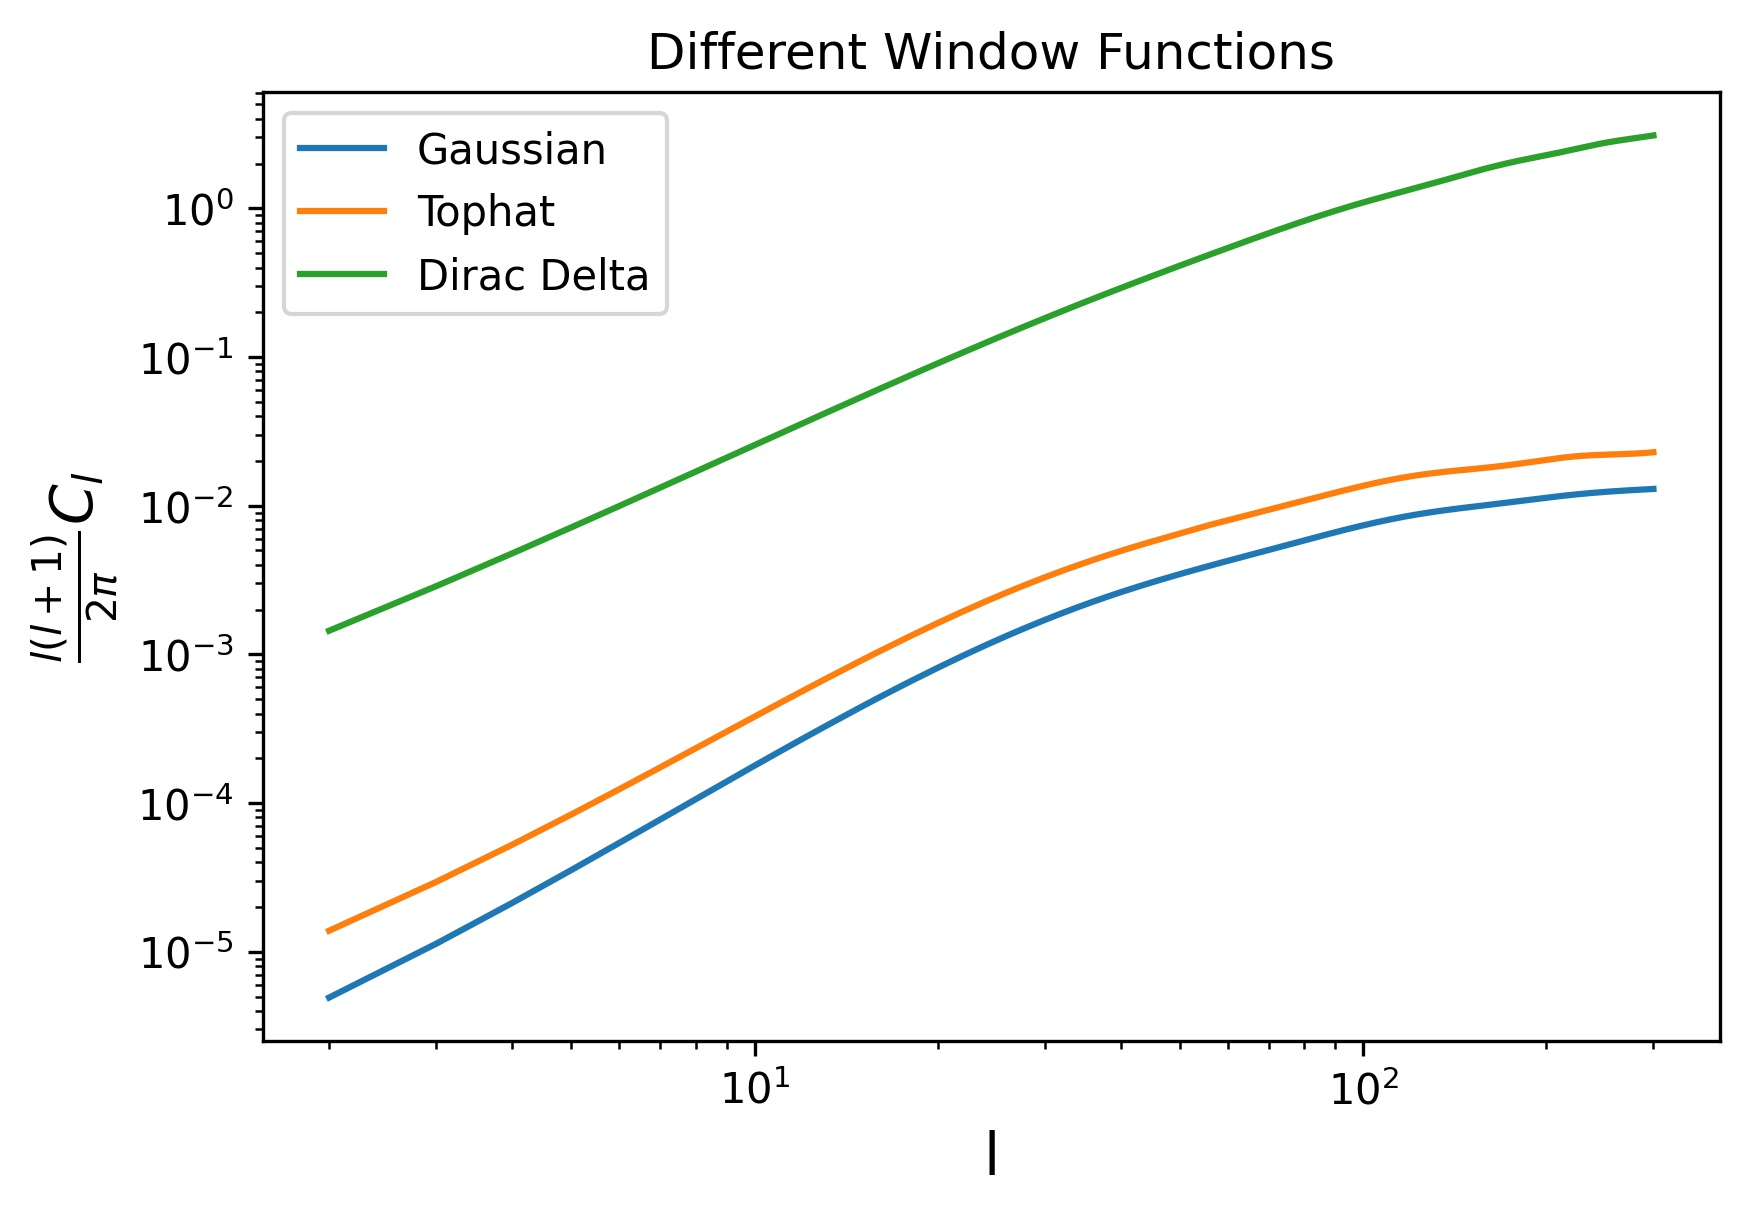
\includegraphics[width=0.7\linewidth]{Images/GW_autocorr_window-fct.jpg}
 \caption{GW angular power spectrum for different window functions}
 \label{plot_Cl_window_fct}
\end{figure} 

\begin{figure}[h]
 \centering
 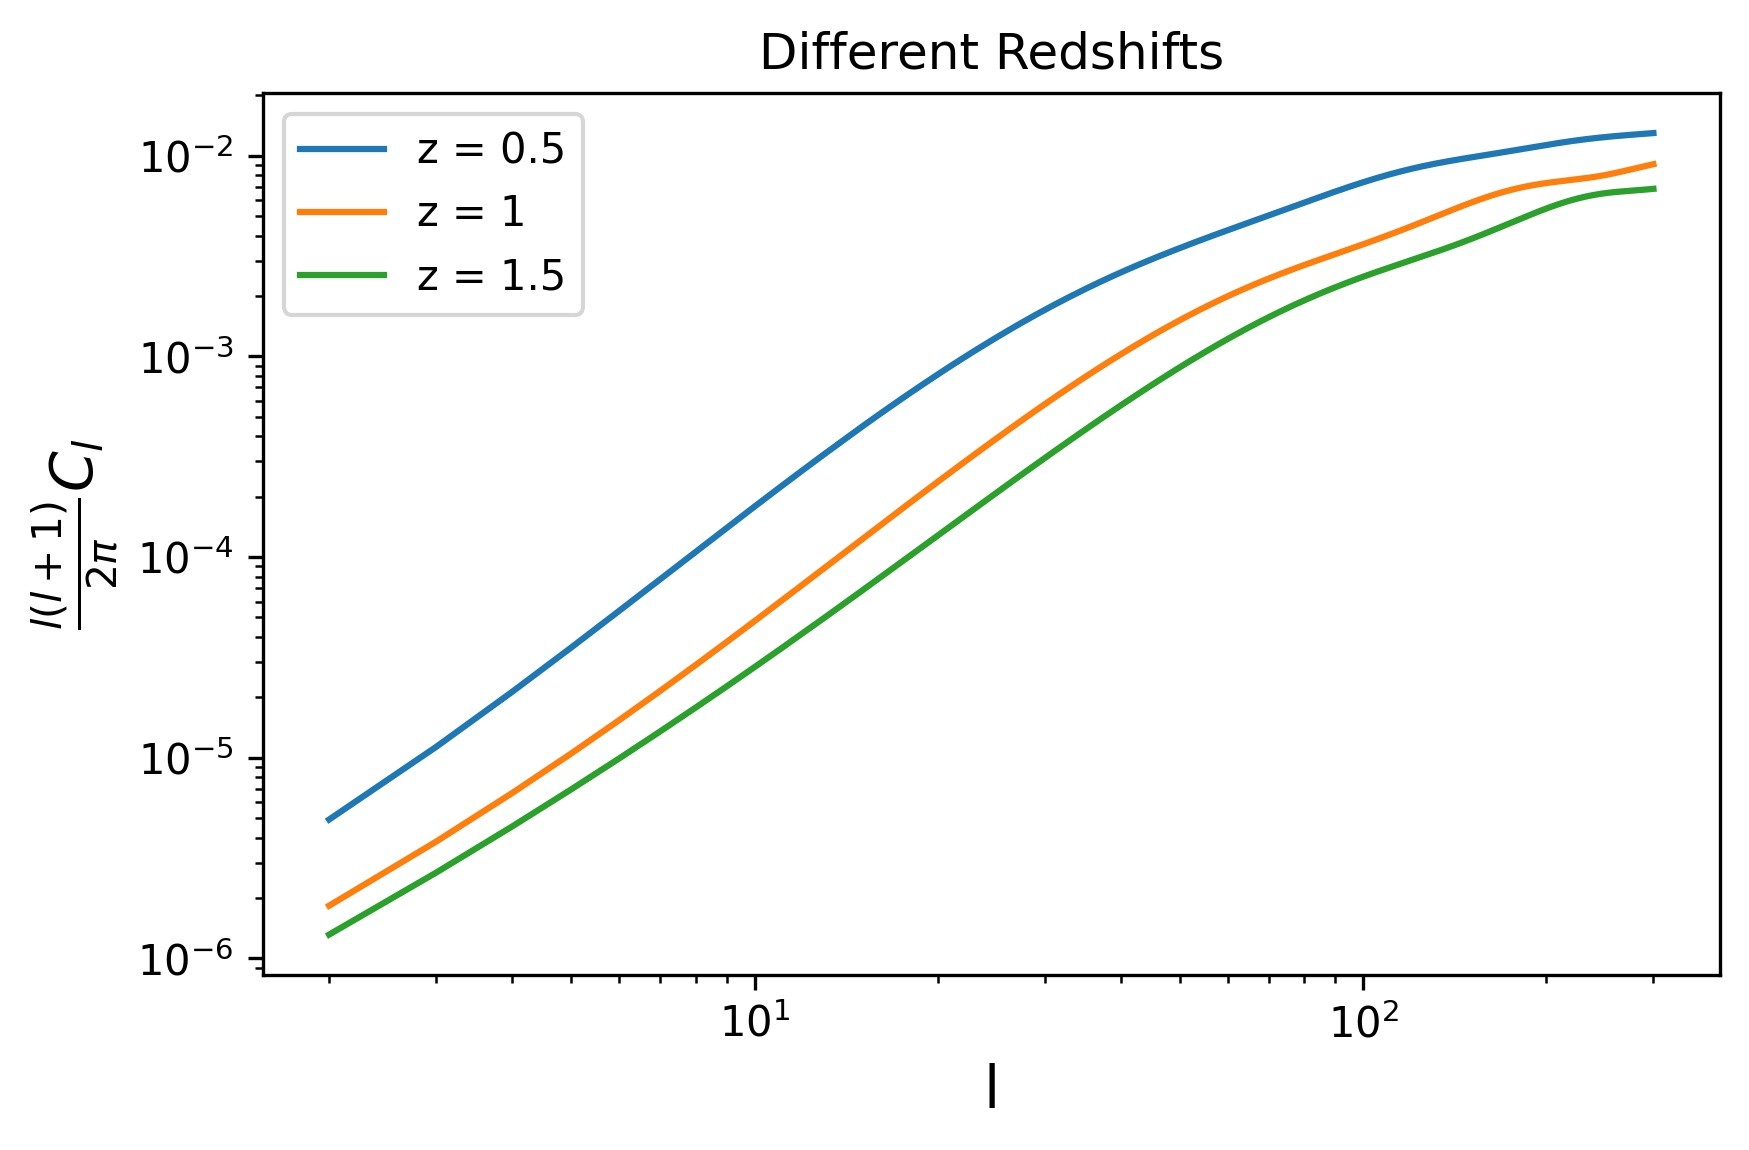
\includegraphics[width=0.7\linewidth]{Images/GW_autocorr_z.jpg}
 \caption{GW angular power spectrum for different redshifts}
 \label{plot_Cl_redshift}
\end{figure} 

As we can see in the Dall'Armi paper the window function and the evolution bias 
depend on the frequency. But this is only the case if we consider not only the
 inspiral phase, but also the merger and ringdown phases. For the inspiral phase
  only, we have the following:
\begin{equation}
    \frac{dE_{GW}}{df_e d\Omega_e} \propto f_0^{-\frac{1}{3}}(1+z)^{-\frac{1}{3}} .
\end{equation}
The window function is proportional to:
\begin{equation}
    \tilde{W}(z)\propto \frac{f_0(E_{GW}/df_e}{\bar{\Omega}_{AGWB}(f_0)} .
\end{equation}

Since we have $\bar{\Omega}_{AGWB}\propto f_0^{\frac{2}{3}}$, considering only 
the inspiral phase would make the window function frequency independent and thus the 
component separation could not work. 


\section{Energy Spectrum}


For the modelling of all three phases we can 
use the waveform by \cite{ajith_inspiral-merger-ringdown_2011}:

\[ A(f) = C f_1^{-7/6} \begin{cases}
        f'^{-7/6}(1+ \sum_{i=2}^3\alpha_i v^i) & f<f_1 \\
        \omega_m f'^{-2/3}(1+ \sum_{i=1}^2 \epsilon_i v^i) & f_1 \leq f < f_2 \\
        \omega_r \mathcal{L}(f, f_2, \sigma) & f_2 \leq f < f_3
\end{cases}
\]

Note that this is the amplitude as a function of the frequency, so a Fourier transform of $A(t)$.

\begin{equation}
    A(f) =  \frac{1}{\sqrt{2\pi}}\int_\mathbb{R} A(t) e^{-ift} dt
\end{equation}

The parameters $\omega_m$ and $\omega_r$ are used to make the function continuous. For the ringdown, we have a Lorentzian function centred around the merger to ringdown transition frequency $f_2$ with the width $\sigma$. The parameters $\alpha_i$ are post-Newtonian corrections.

\begin{table}[h]
    \begin{center}
        \begin{tabular}{ c | c | c | c | c}
            Parameter & $\alpha_2$ & $\alpha_3$ & $\epsilon_1$ & $\epsilon_2$ \\
            \hline
            Value & -323/224 + 451$\eta$/168 & (27/8-11$\eta$/6)$\chi$ & 1.455$\chi$-1.890 & -1.815$\chi$ + 1.656\\
            \hline
            No Spin & -323/224 +  451$\eta$/168 & 0 & -1.890 & 1.656 
        \end{tabular}
        \caption{Amplitude parameters with and without the zero spin approximation.}
        \label{amplitude_param}
    \end{center}
\end{table}

The frequency $f_1$ at the transition of the inspiral and merger phase is the last stable orbit of the binary. Once the merger phase has started the orbits cease to be stable since the objects start to fall in. This frequency was calculated by \cite{bardeen_rotating_1972}.

\begin{equation}
    f_1 = \frac{c^3}{6^{3/2}2\pi M_{tot} G}
\end{equation}

The transition frequency from merger to ringdown is given by the least-damped mode (\cite{maggiore_gravitational_2008}) which is also the dominant quasi-normal mode. This is part of the description of the BBH system as characterised by n normal modes with frequencies $\omega_n$, discussed further in chapter 12.3 of the same book.

\begin{equation}
    f_2 \approx 0.747 \frac{c}{2\pi R_S} \approx 12 \rm{kHz} \left( \frac{M_\odot}{M}\right)
\end{equation}

Later, we will consider the square strain as a function of frequency $|h(f)|^2$ for the energy spectrum, so we can ignore the phase $\psi(f)$.

\begin{equation}
    h(f)=A(f)e^{-\psi(f)}
\end{equation}

Here the redshift dependence will come in through the derivation by the emission 
frequency, see e.g. \ref{window}. From this waveform template, we can get the energy 
spectrum in the following way.
\begin{equation}
    \frac{dE_{GW,e}}{df_e d\Omega_e} = \frac{\pi d_L^2 c^3f_0^2}{2G(1+z)^2}
    \mid h(f_0)\mid ^2
\end{equation}

\begin{figure}
    \centering
    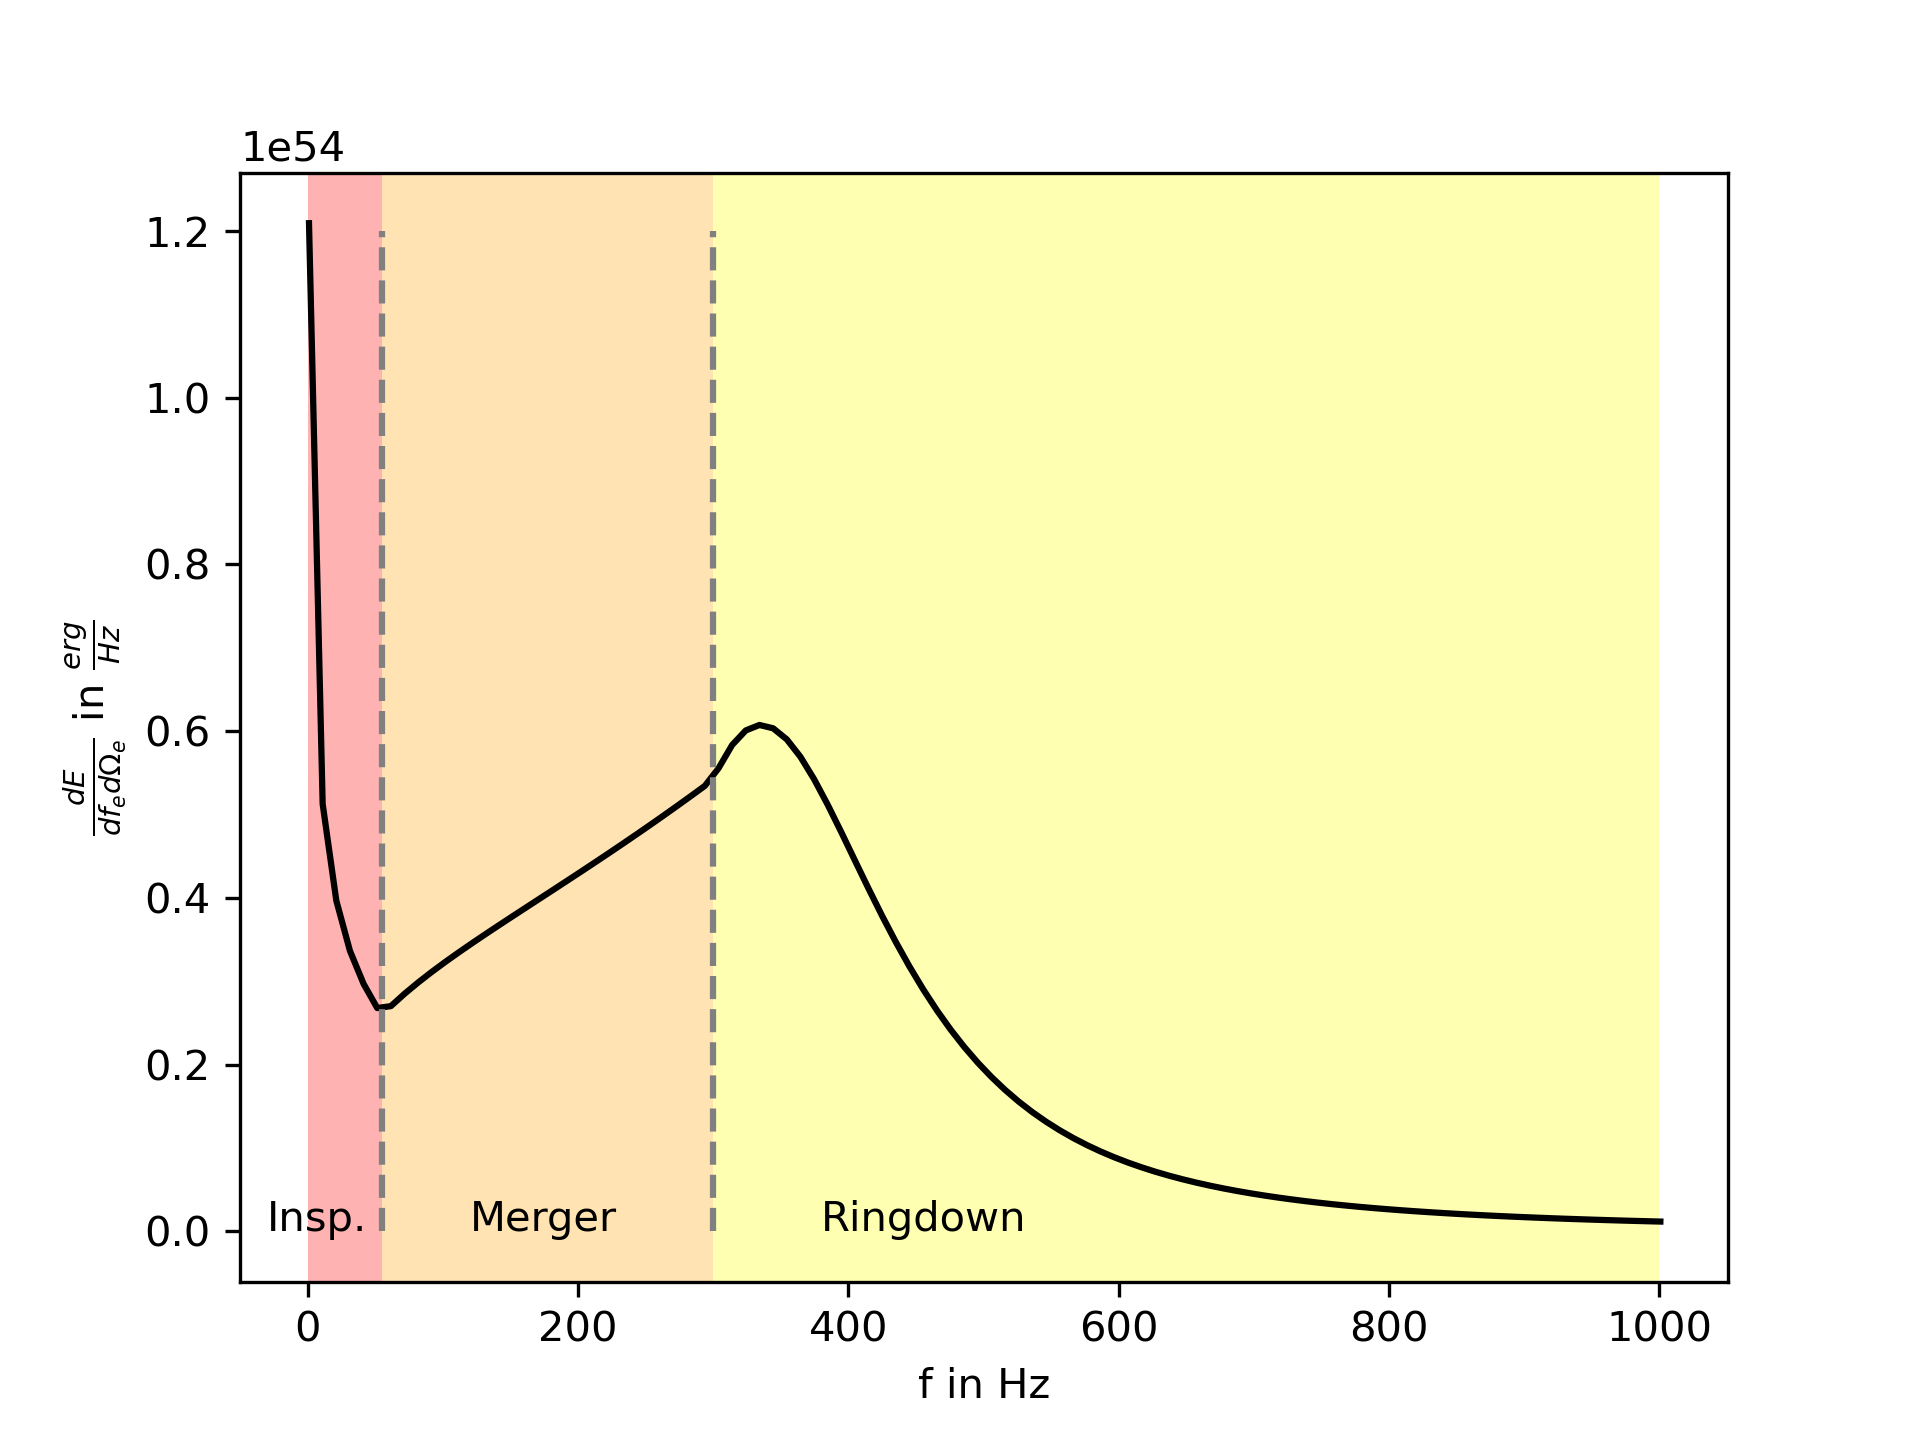
\includegraphics[width=1\linewidth]{Images/dE_df_of_f.png}
    \caption{The energy spectrum as a function of frequency for a BBH merger, where both BH have a mass of 20$M_\odot\ $. }
    \label{dE_df_f}
\end{figure} 

%\vspace{-5cm}
\begin{figure}
    \centering
    \subfloat[The energy spectrum at an observed frequency \newline of 1 Hz]{
        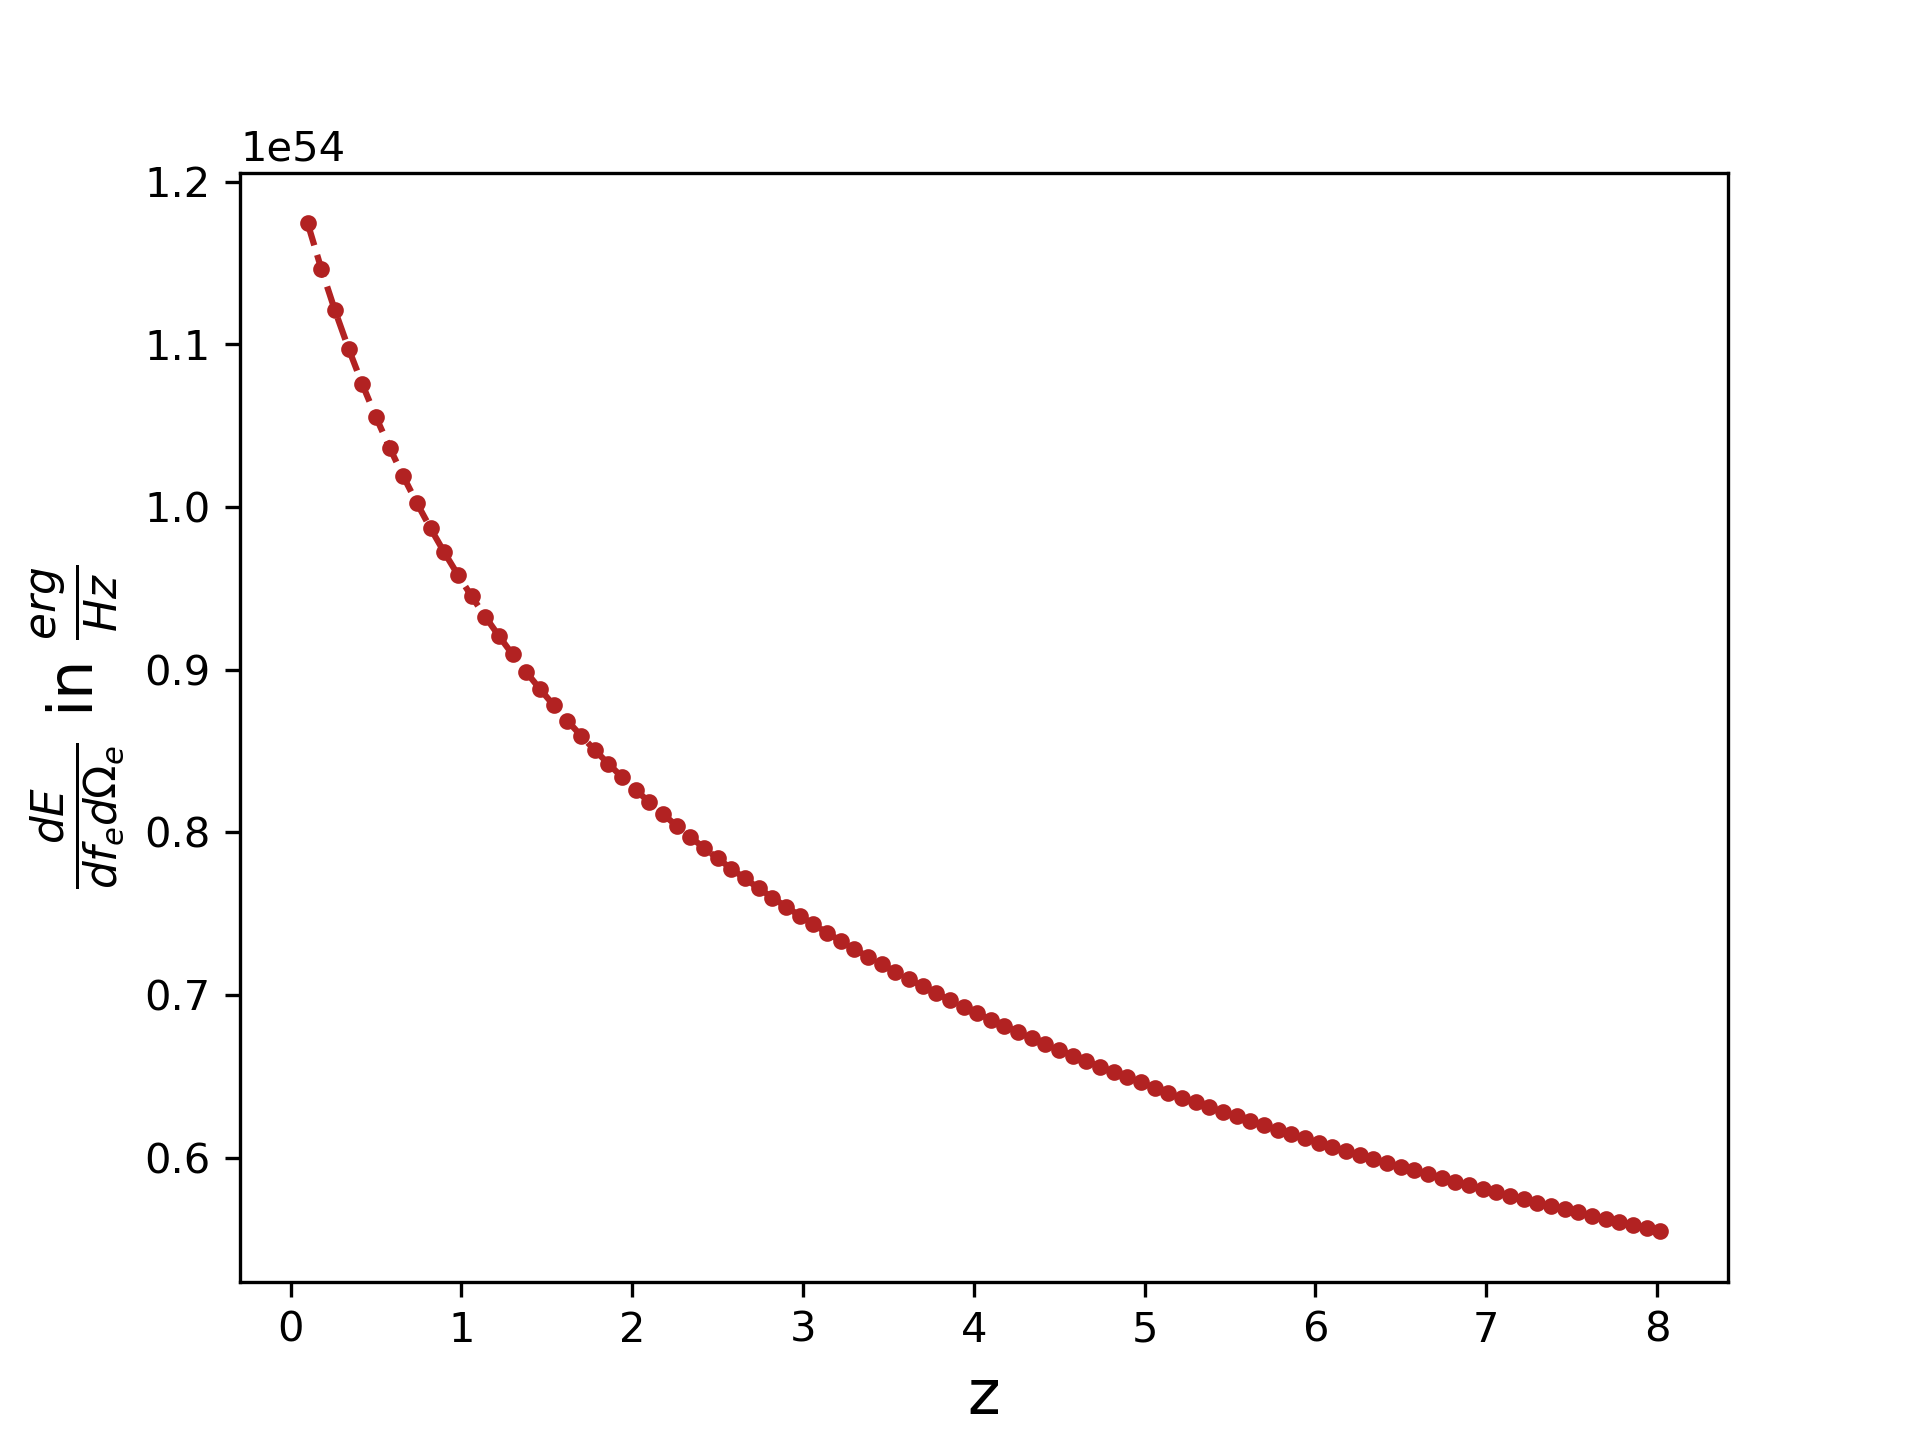
\includegraphics[width=7.5cm, clip]{Images/E_spectrum_z_1Hz.png}}
    %\hspace{1.00\baselineskip}
    \subfloat[The energy spectrum at an observed frequency \newline of 10 Hz]{
        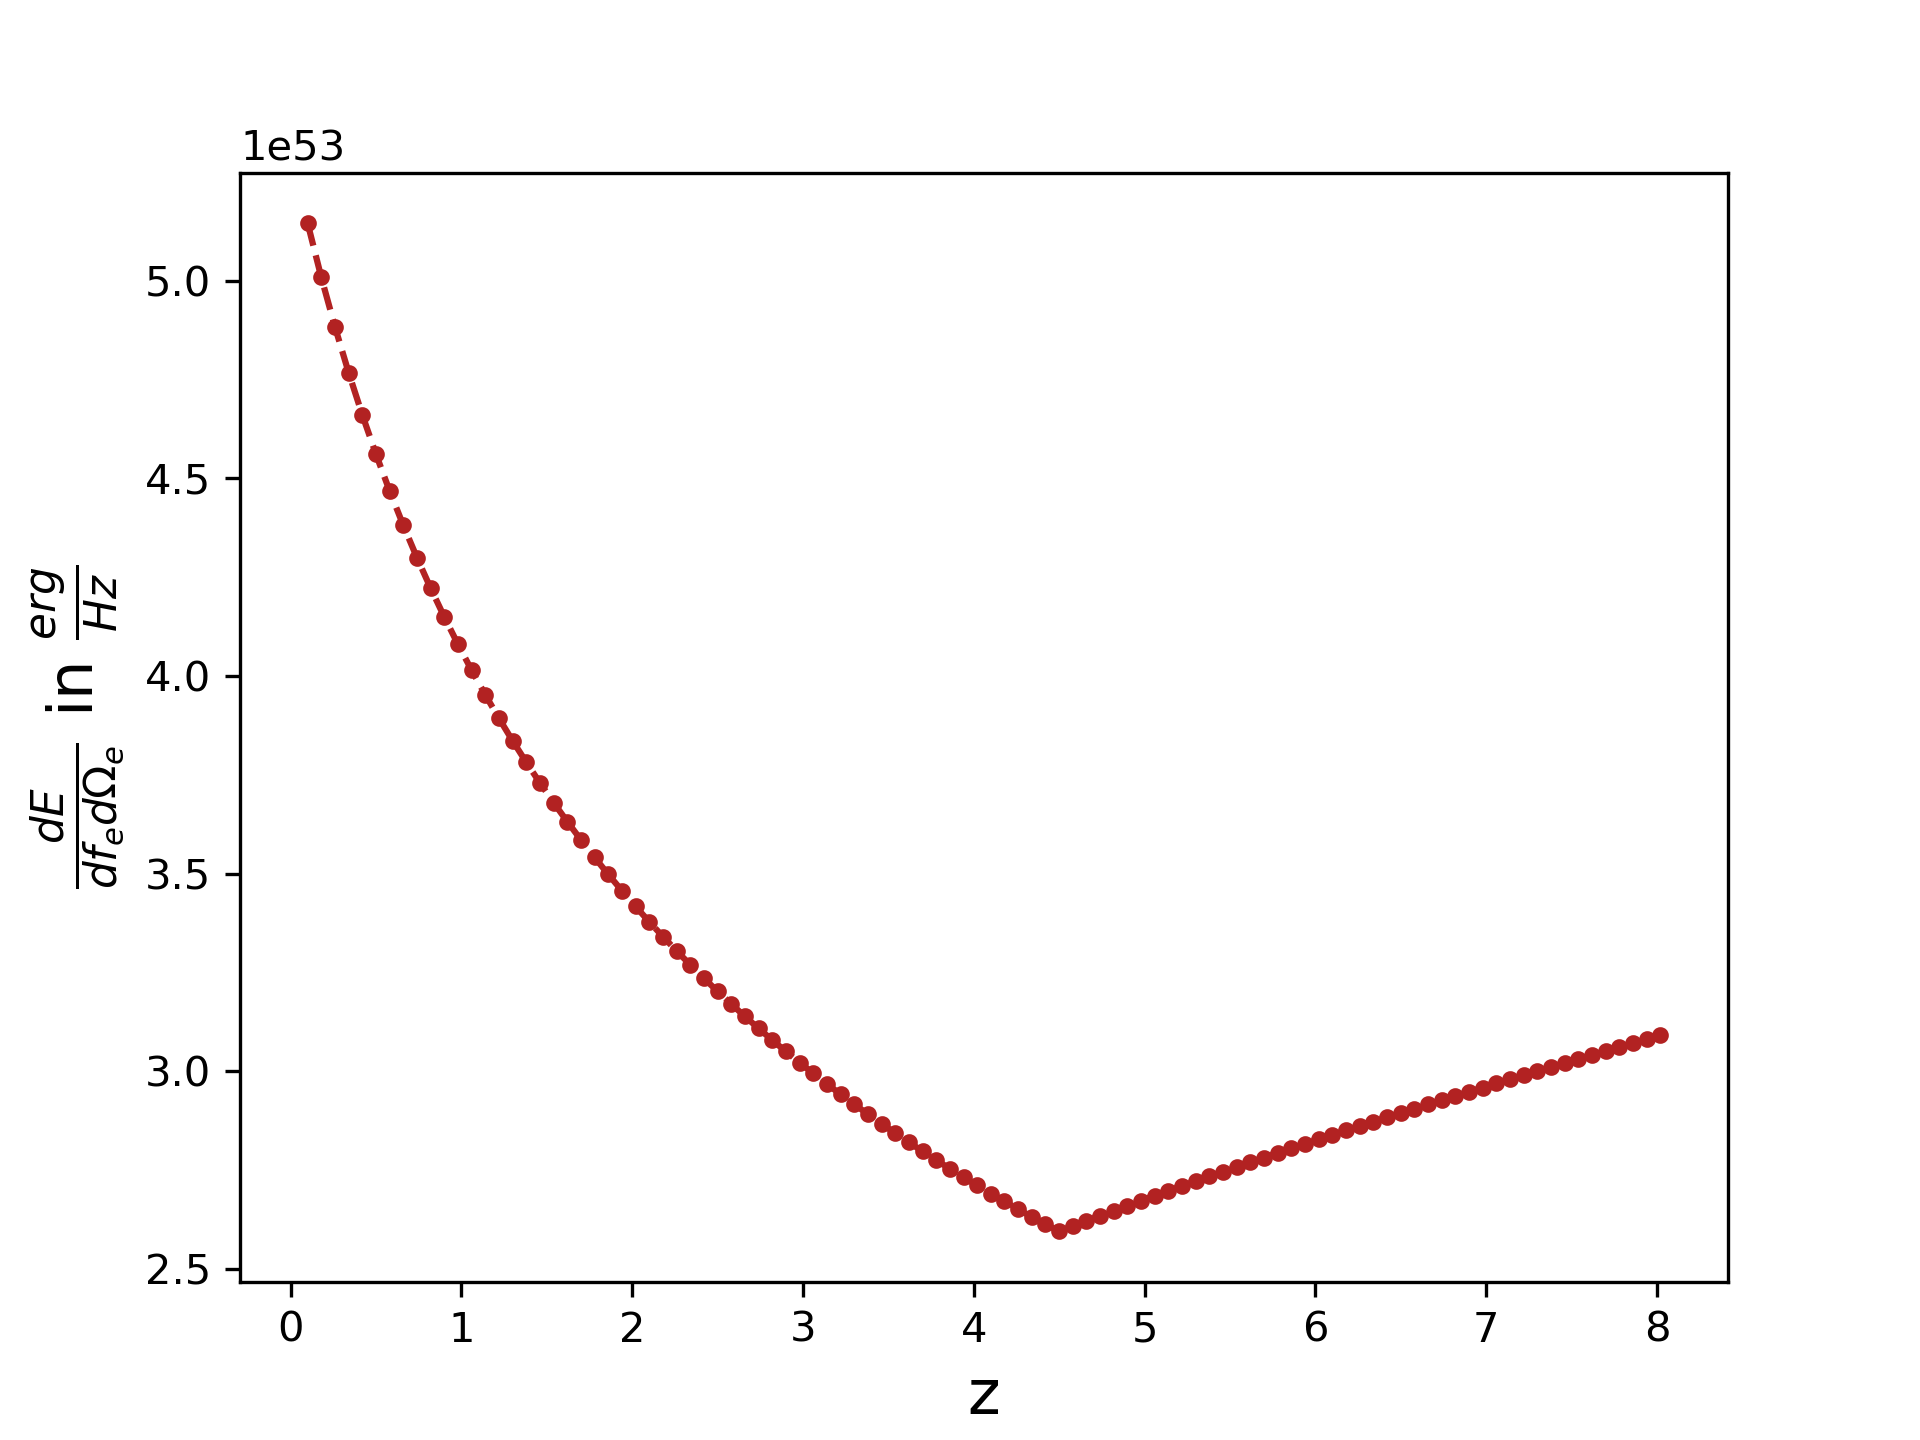
\includegraphics[width=7.5cm, clip]{Images/E_spectrum_z_10Hz.png}}
    \\
    %\vspace{-1.00\baselineskip}
    \subfloat[The energy spectrum at an observed frequency \newline of 100 Hz]{
        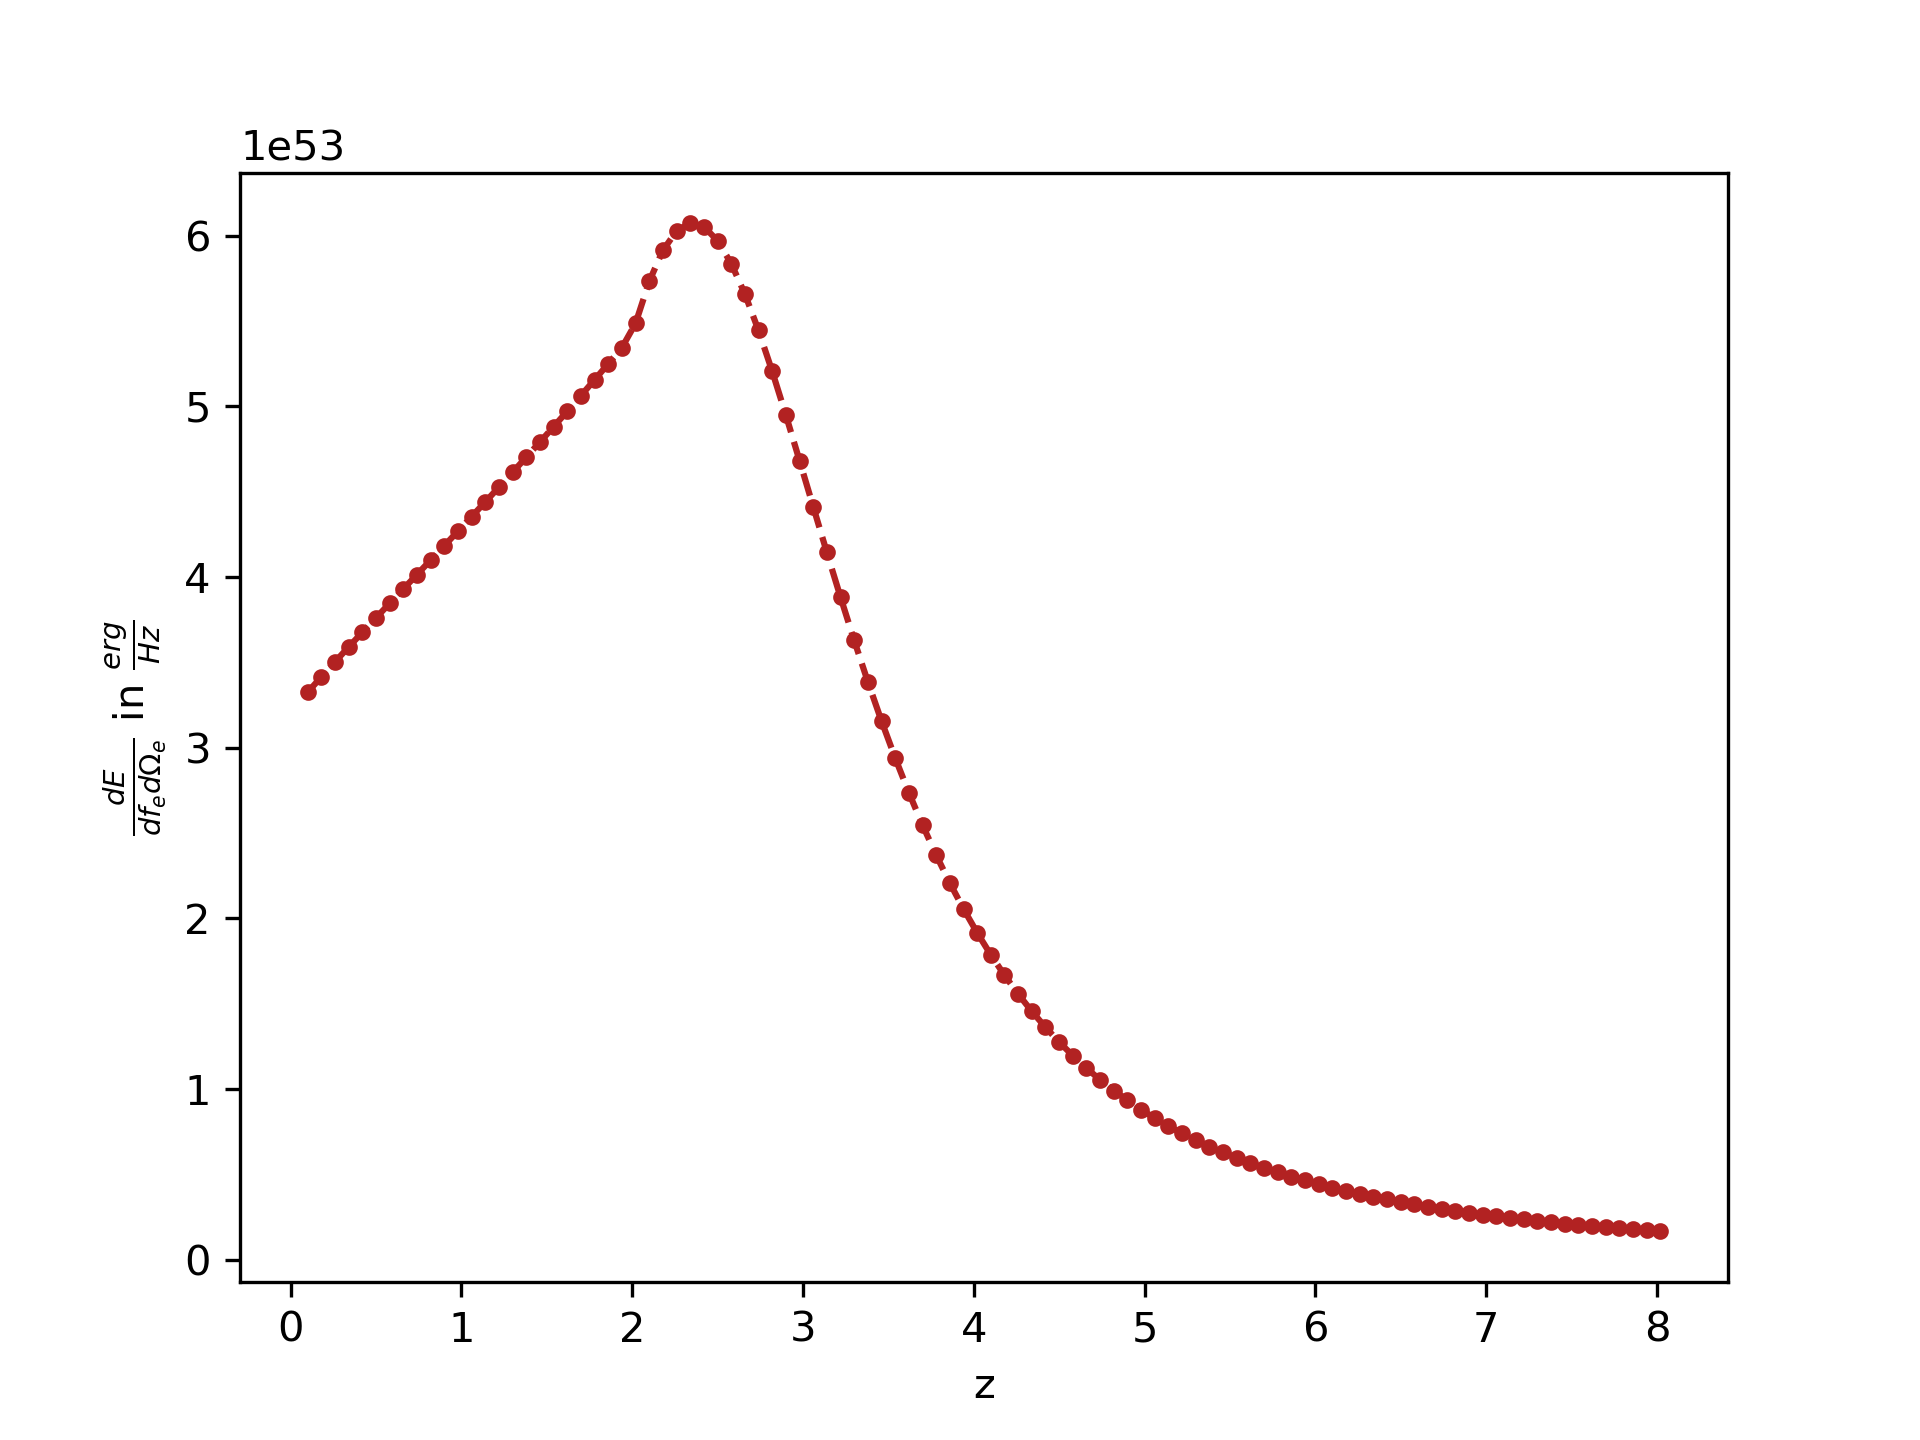
\includegraphics[width=7.5cm, clip]{Images/E_spectrum_z_100Hz.png}}
    %\hspace{-2.00\baselineskip}
    \subfloat[The energy spectrum at an observed frequency \newline of 1000 Hz]{
        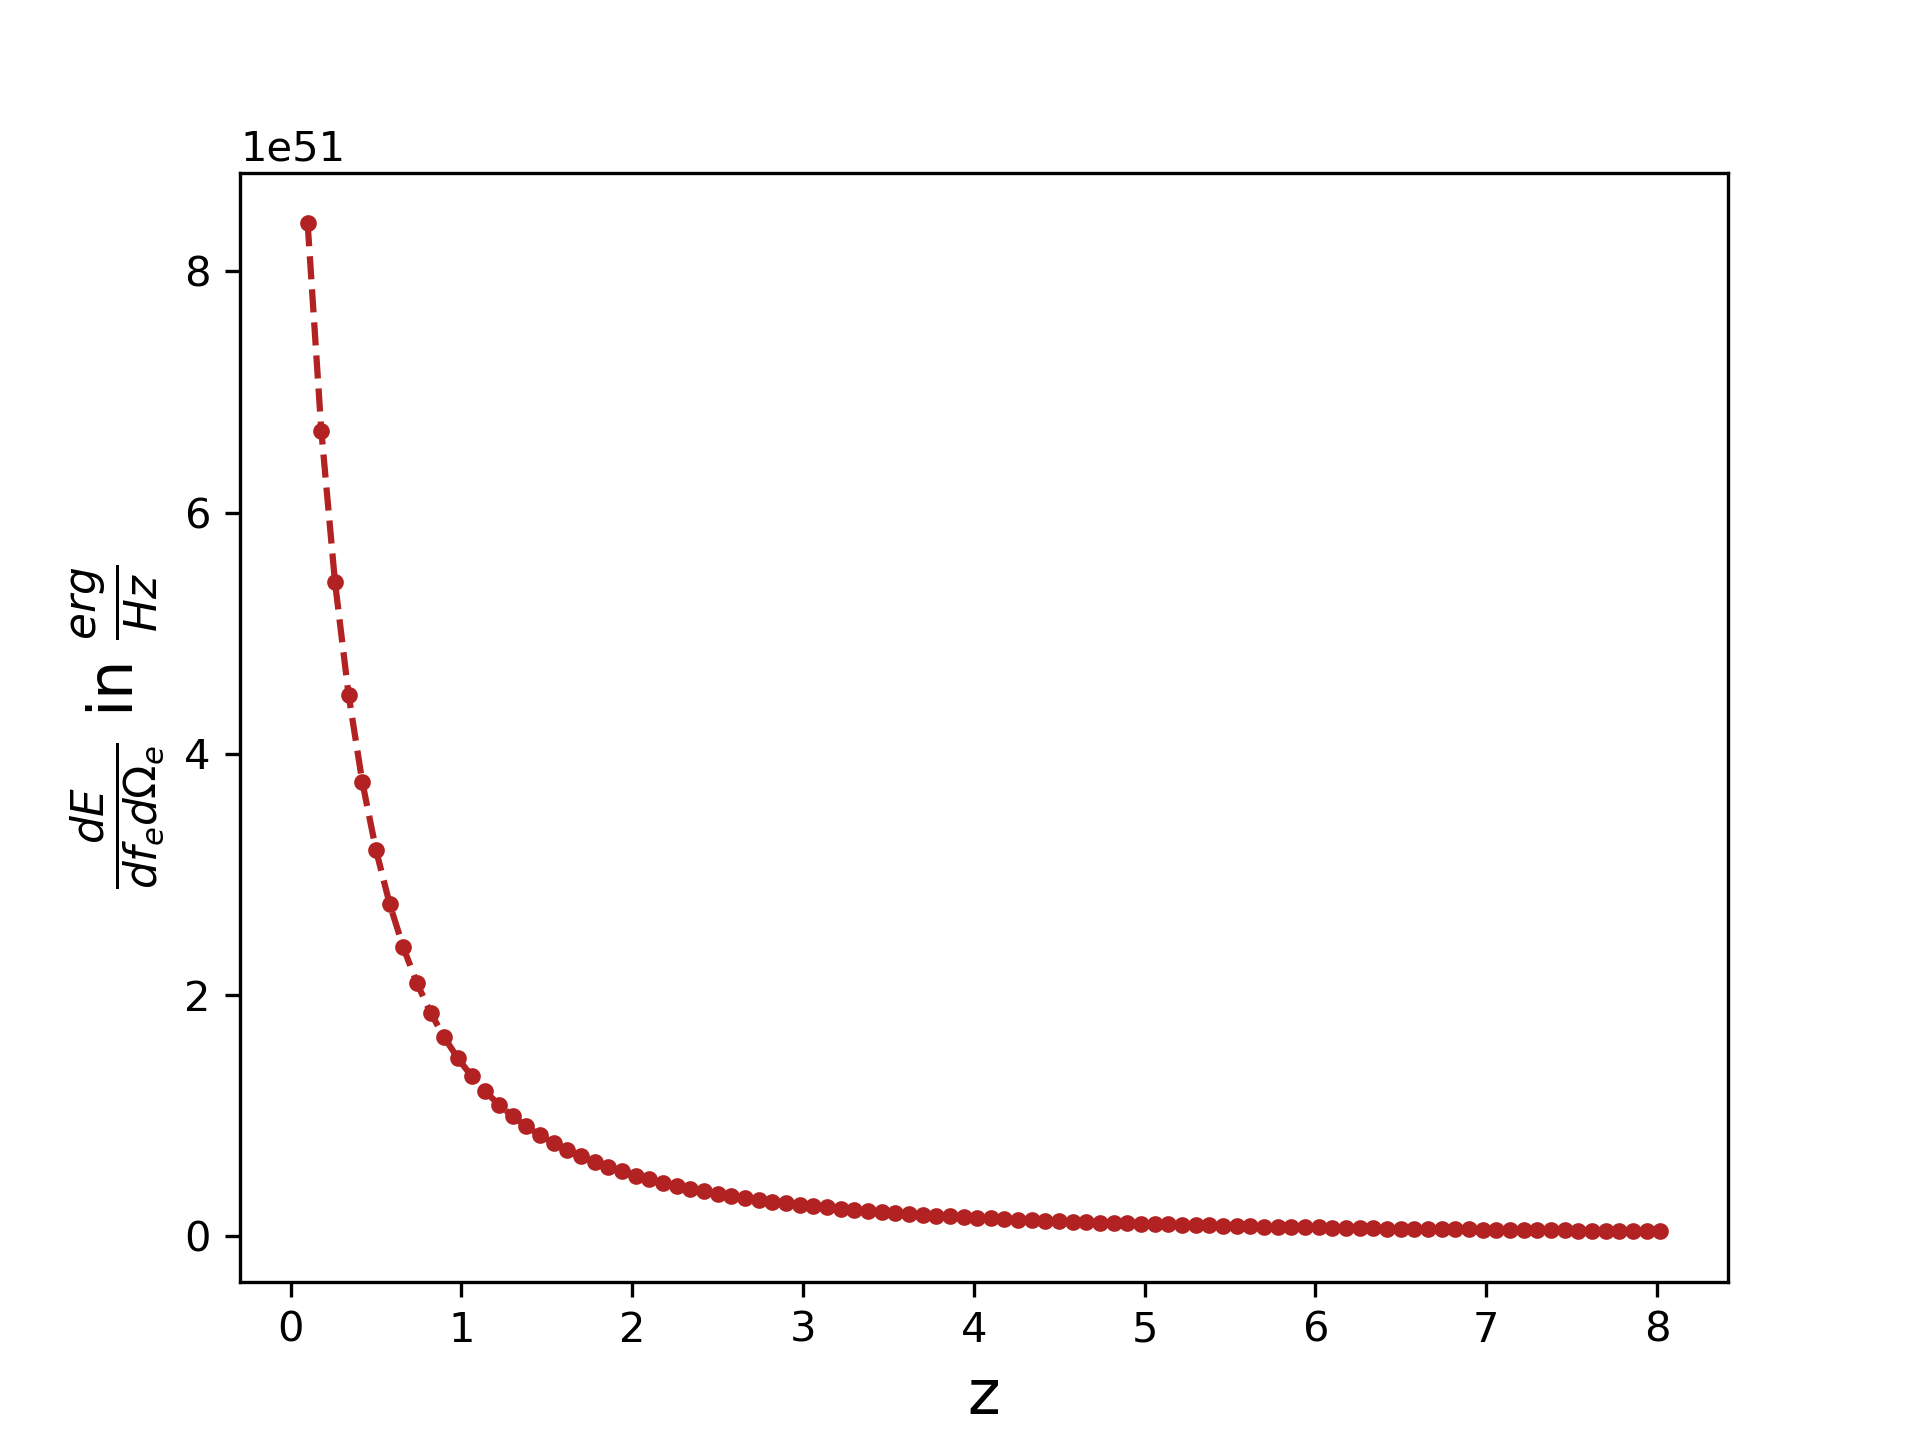
\includegraphics[width=7.5cm, clip]{Images/E_spectrum_z_1000Hz.png}}
  
    \caption{The energy spectrum $\frac{d^2E}{df_e d\Omega_e}$ at different observed freqeuncies as a function of redshift.}
    \label{dE_df_diff_frequencies}
\end{figure}

If we plot the energy spectrum as a function of z for different frequencies, see Fig. \ref{dE_df_diff_frequencies}, we can see different sections of Fig. \ref{dE_df_f}. This is because $d^2 E_{GW,e}/df_e d\Omega_e$ only depends on z through the emitted frequency. The energy spectrum is written as a function of $f_e$, but we implement it in such a way that the user can choose the received frequency at the detector.


\begin{equation}
    f_e = (1+z)f_0
\end{equation}

\section{Merger Rate}
\begin{equation}
    R_{BBH}(z=0) = 19 \:\rm{Gpc}^{-3}\rm{yr}{-1}
\end{equation}
\begin{equation}
    R_{BBH}(z)=\mathcal{A}_{LIGO}^{BBH}\int dt_d p(t_d) \int dM_h \frac{dn}{dM_h}(z_f, M_h)\langle SFR(M_h, z_f)\rangle_{SF}
    \label{BBH_merger_equation}
\end{equation}

Here, we have the time delay distribution $p(t_d)$, where the time delay is between the formation and the merger of the binary. (physical explanation)

For the merger rate of binary black holes, we need the star formation rate. 

...

\begin{figure}[h]
    \centering
    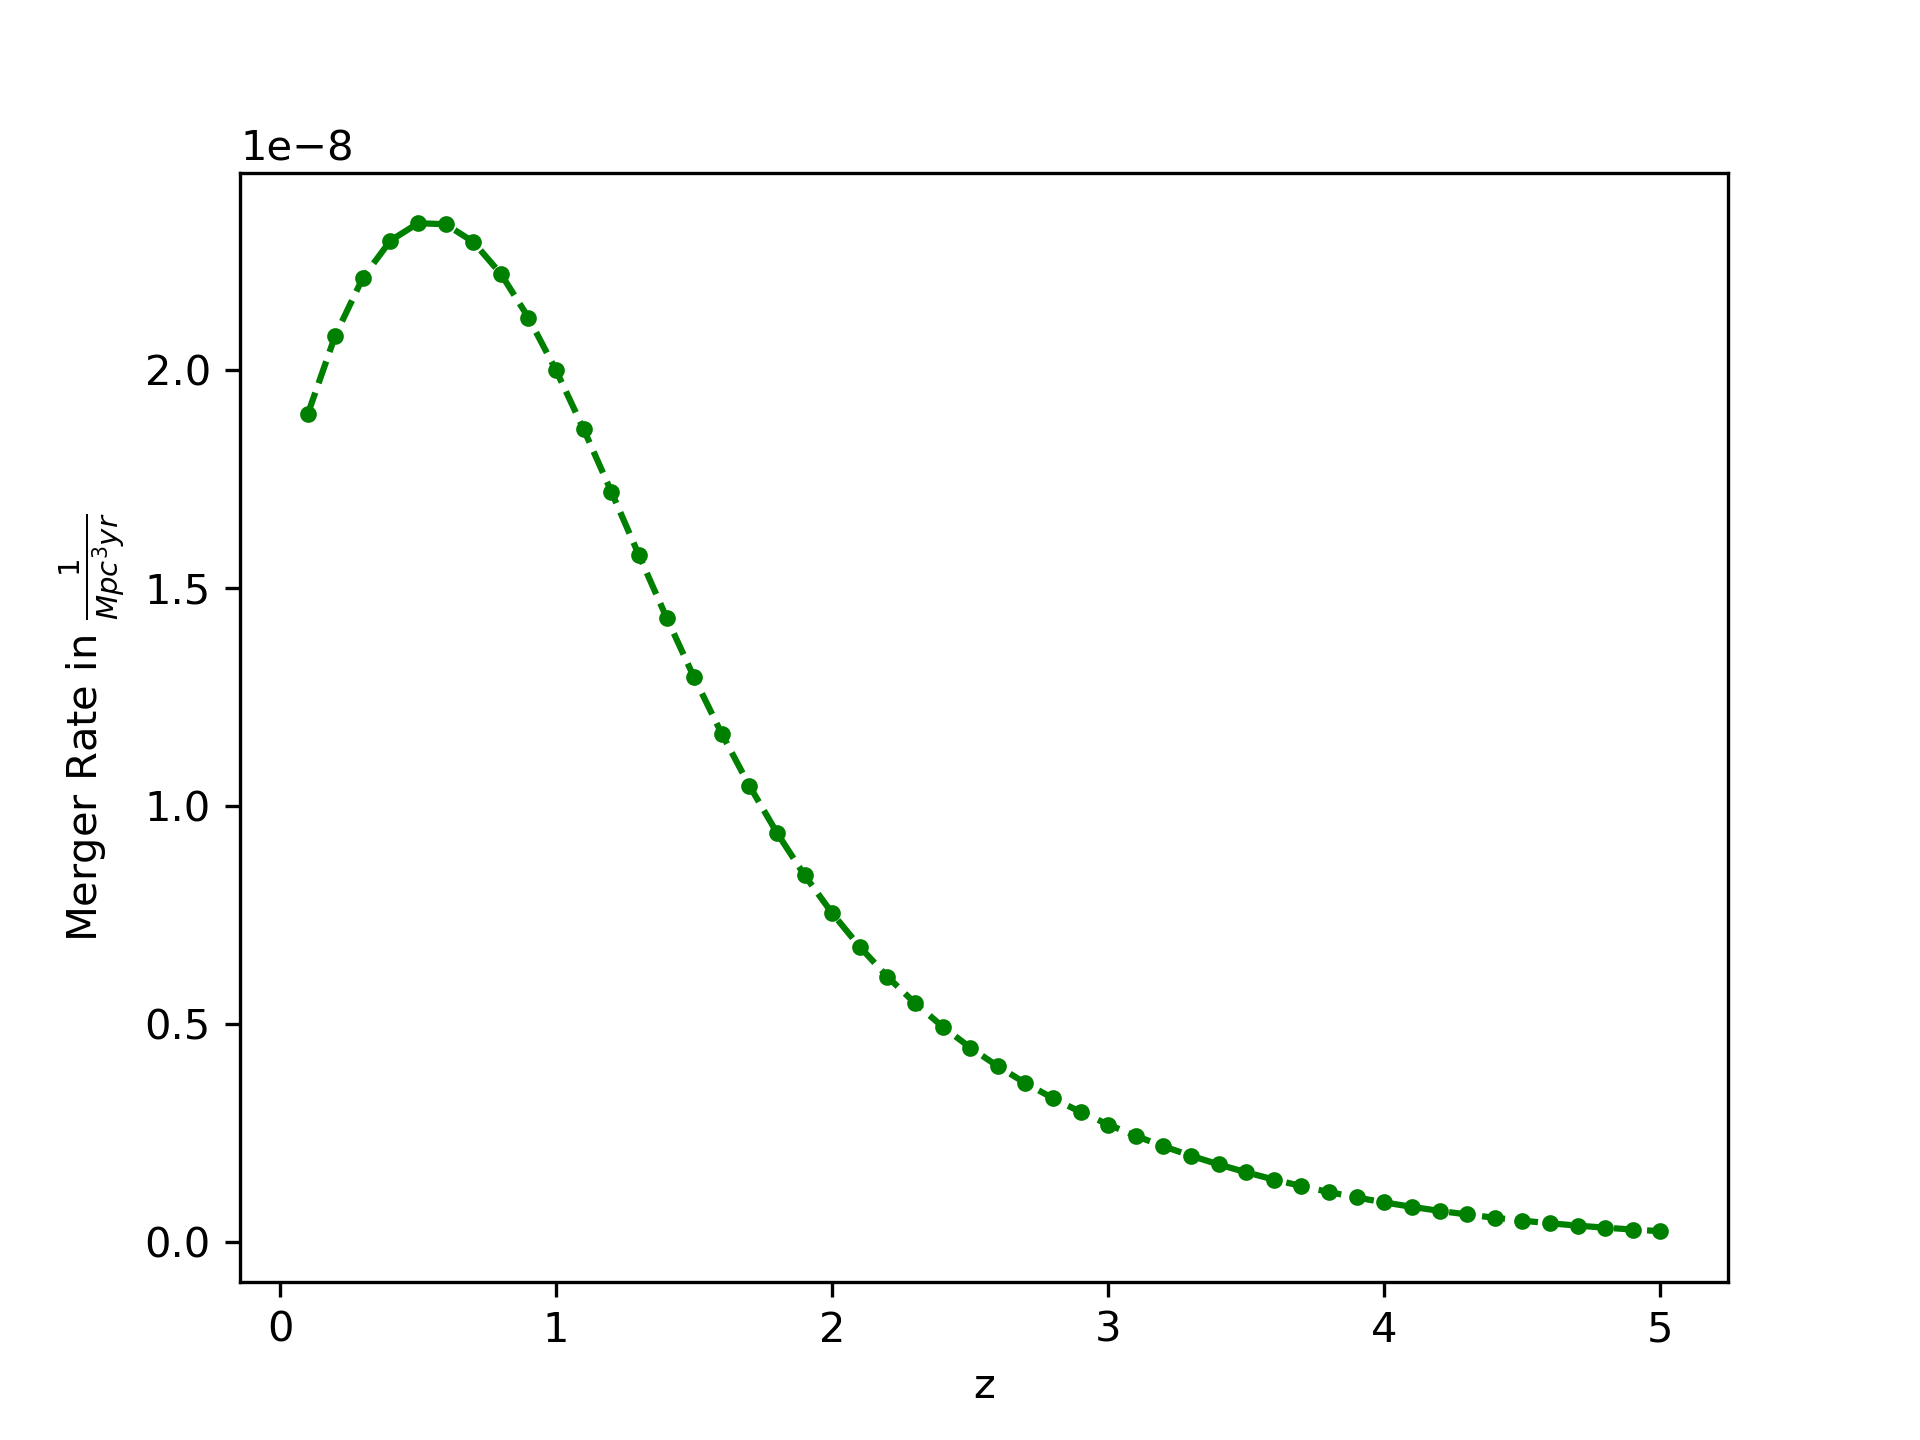
\includegraphics[width=1\linewidth]{Images/bbh_merger_rate.png}
    \caption{BBH merger rate as a function of the redshift z}
    \label{bbh_merger_rate}
   \end{figure} 

\section{Star Formation Rate}
\subsection{\textsc{UniverseMachine}}

For the star formation rate, we use the \textsc{UniverseMachine} code from \cite{behroozi_universemachine_2019}. They use observational constraints and data from simulations to compute SFR for individual galaxies. \\

In the $\Lambda$CDM cosmology, galaxies form at the centre of haloes. Haloes are gravitationally self-bound structures that contain virialised dark matter. This means that the virial equation applies in this case. Here, $T$ is the potential energy and $U$ is the kinetic energy.

\begin{equation}
    2T=U
\end{equation}

So far, there exists no framework in which we can derive the SFR from first principles. This is why the authors use a double power law plus Gaussian and determine the best-fit parameters for this functional form. This determines the SFR for every halo at a given redshift. They use weak priors and observational constraints for less bias and the potential to reveal new physics.

Dark matter simulations, here Bolshoi-Planck [\cite{klypin_dark_2011}] and MultiDark Planck 2 (MDPL2) \cite{klypin_multidark_2016}, are used, which simulate a mock universe. They contain halo merger trees, which can be compared to observations. Behroozi et al. used data from multiple experiments, such as the Sloan Digital Sky Survey (SDSS) \cite{abazajian_seventh_2009}, Ultravista \cite{mccracken_ultravista_2012}. The observables include stellar mass functions, UV luminosity functions and galaxy auto-correlation functions.
Using this data, they compute a likelihood and run a Markov Chain Monte Carlo (MCMC) algorithm to sample the SFR range.

Like in \cite{dallarmi_dipole_2022} we consider only star-forming galaxies. This could be modified in a future version of the code by including the fraction of quenched galaxies $f_Q = 1 -f_{SF}$, which could be taken from the \textsc{UniverseMachine} paper as well. The adopted SFR functional form is the following.

\begin{equation}
    SFR_{SF} = \epsilon \left[ \left( v^\alpha + v^\beta \right)^{-1} + \gamma \exp \left(-\frac{\log_{10}(v)^2}{2\delta^2}\right) \right]
\end{equation}

The characteristic SFR  in $M_\odot\ yr^{-1}$ is the global factor $\epsilon$. For the slope of the $SFR-v_{Mpeak}$ relation, we have a faint-end and a massive-end slope parameter $\alpha$ and $\beta$, respectively. This is because $v_{Mpeak} \propto M_h^3$ \ref{v_mpeak-M_h-relation}, so a higher velocity at the peak mass corresponds to a higher halo mass.
Furthermore, $\gamma$ is the strength and $\delta$ the width of the Gaussian SFR efficiency boost. 

The velocity $v$ is defined as the ratio of the real ($v_{Mpeak})$ and the characteristic ($V$) velocity at the halo peak mass, both in $km s^{-1}$.

\begin{equation}
    v = \frac{v_{Mpeak}}{V \cdot km s^{-1}}
\end{equation}

The other parameters, except for $\delta$, scale differently for different redshift regions. For $V$, $\epsilon$ and $\alpha$, the scaling is separated into $z=0$, $z\approx 1-2$, $z=3-7$ and $z>7$. The parameters $\beta$ and $\gamma$ have three scaling regions instead of four, as they are not well constrained at high redshifts. 

\begin{equation}
    \log_{10}(V) = V_0 + V_a(1-a)+V_{la}ln(1+z)+V_z z
\end{equation}
\begin{equation}
    \log_{10}(\epsilon) = \epsilon_0 + \epsilon_a(1-a)+\epsilon_{la}ln(1+z)+\epsilon_z z
\end{equation}
\begin{equation}
    \alpha = \alpha_0 + \alpha_a(1-a)+\alpha_{la}ln(1+z)+\alpha_z z
\end{equation}
\begin{equation}
    \beta = \beta_0 + \beta_a(1-a)+\beta_z z
\end{equation}
\begin{equation}
    \log_{10}(\gamma) = \gamma_0 + \gamma_a(1-a)+\gamma_{la}ln(1+z)+\gamma_z z
\end{equation}
\begin{equation}
    \delta = \delta_0
\end{equation}

The median $v_{Mpeak}$ is taken from the \textit{Bolshoi-Planck} DM simulation as

\begin{equation}
    v_{Mpeak}(M_h, a) = 200 \frac{km}{s}\left[ \frac{M_h}{M_{200kms}(a)}\right]^3
    \label{v_mpeak-M_h-relation}
\end{equation}
\begin{equation}
    M_{200kms}(a) = \frac{1.64 \cdot 10^{12} M_\odot\ }{()\frac{a}{0.378})^{-0.142}+(\frac{a}{0.378})^{-1.79}} .
\end{equation}


\begin{figure}[h]
    \centering
    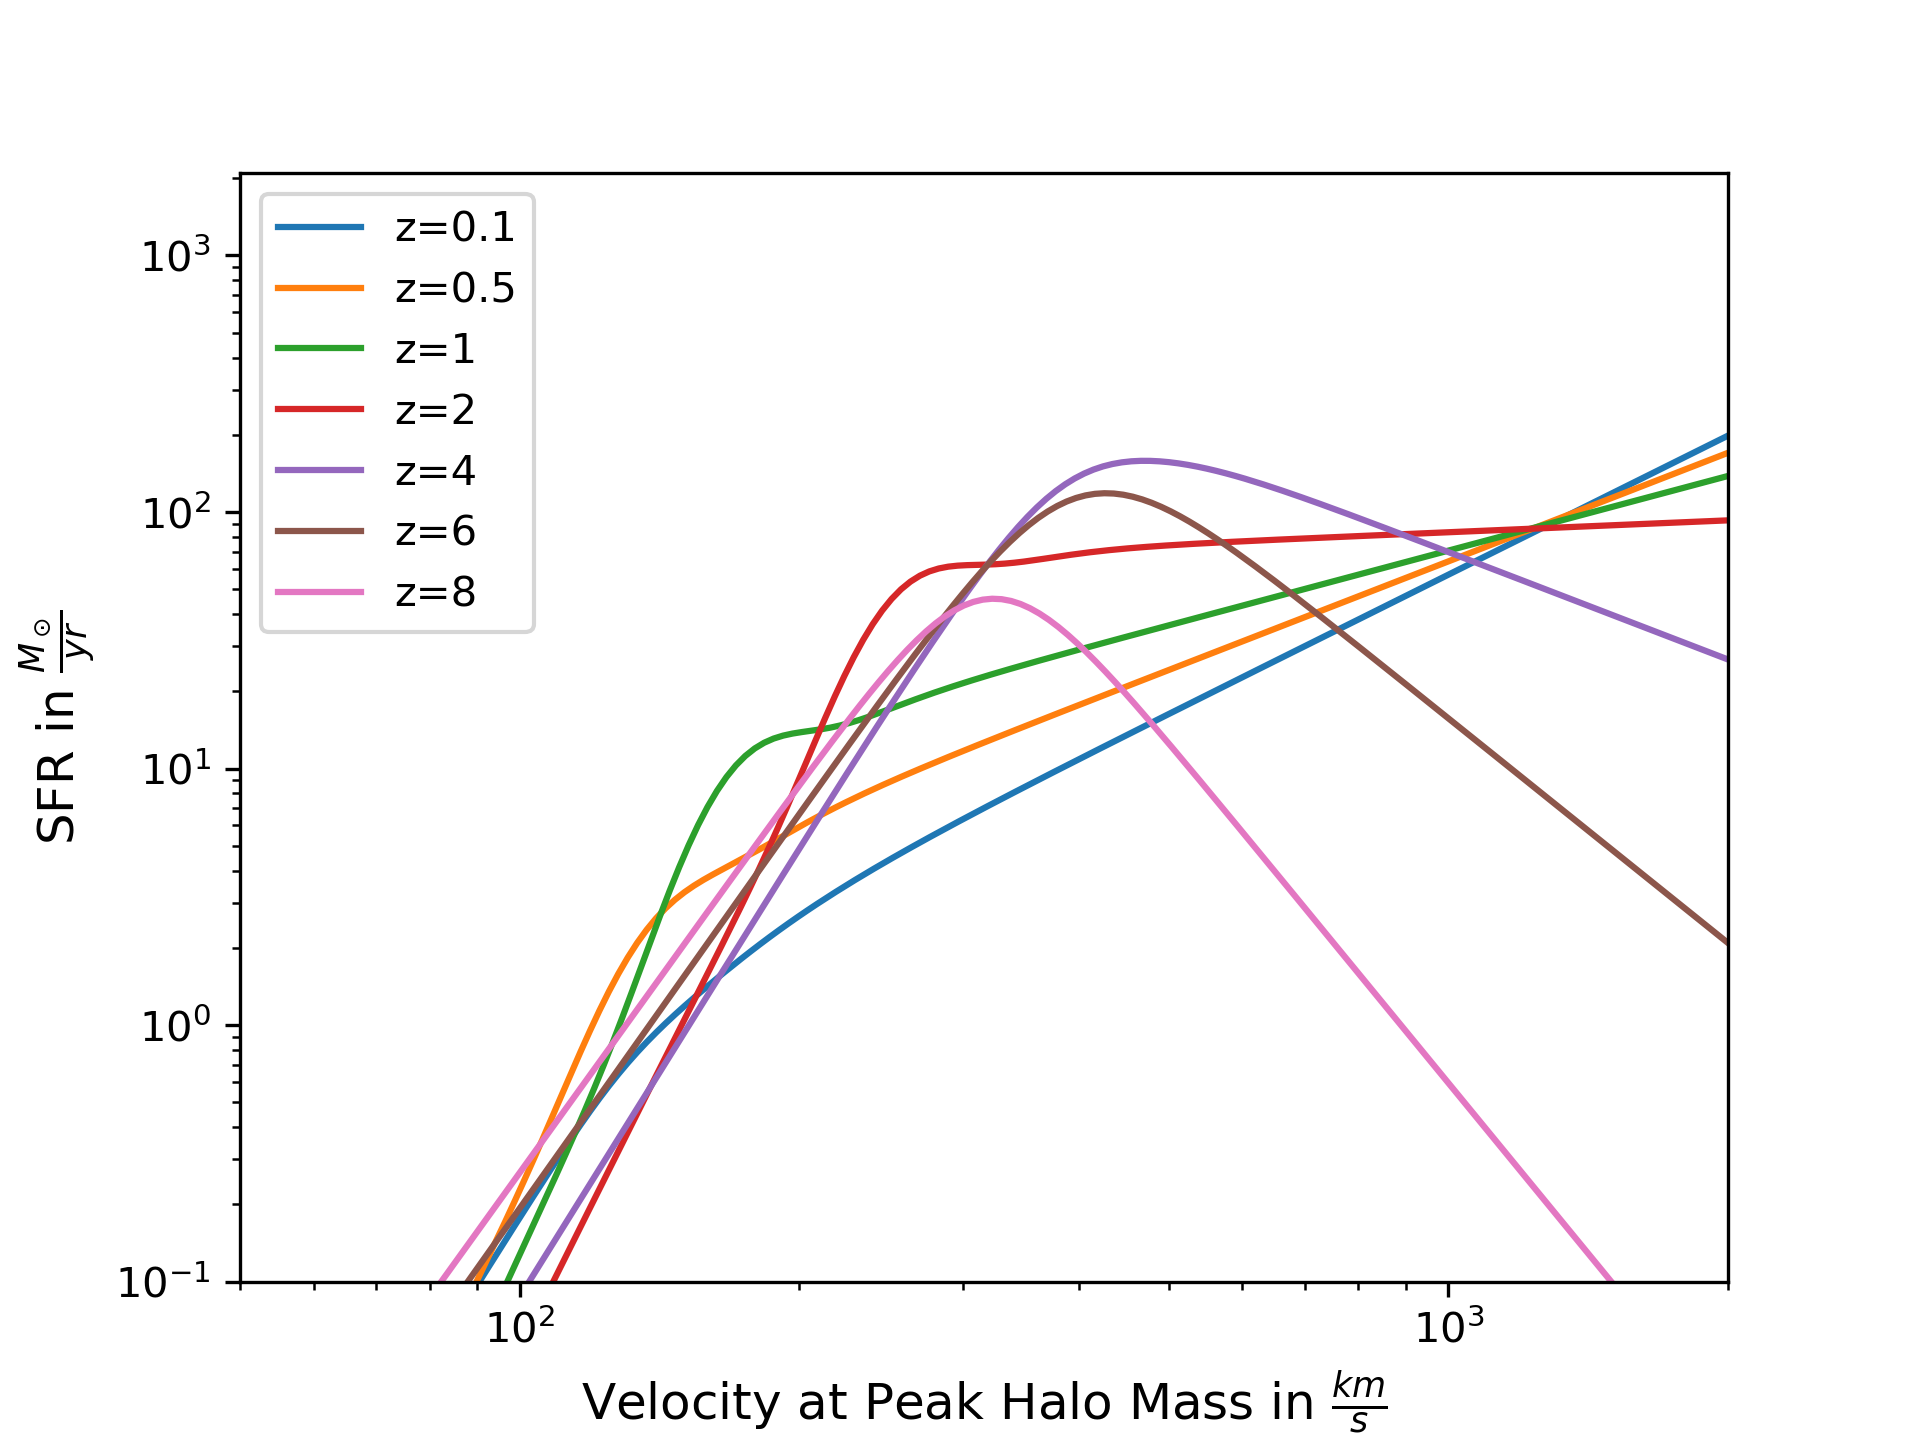
\includegraphics[width=1\linewidth]{Images/sfr_of_v.png}
    \caption{SFR for star-forming galaxies for different redshifts. The velocity at the historical peak halo mass corresponds to the standard halo mass, see equation \ref{v_mpeak-M_h-relation}.}
    \label{SFR_of_v}
\end{figure} 

\section{Halo Mass Function}

\textit{change style}

Since we also need the halo mass function (HMF) to calculate the BBH merger rate, 
see \ref{BBH_merger_equation}. The HMF $dn/dM_h (z_f, M_h)$ was implemented by Daniel Meinert in the "21cm" branch in {\tt CLASS}. It uses the Press-Schechter formalism.

\subsection{Press-Schechter Formalism}

\begin{figure}[h]
    \centering
    \subfloat[The halo mass function in units of $\frac{h/M_\odot}{(Mpc/h)^3}$ or respectively $\frac{h^4}{M\odot Mpc^3}$
        \label{HMF_plot}]{
        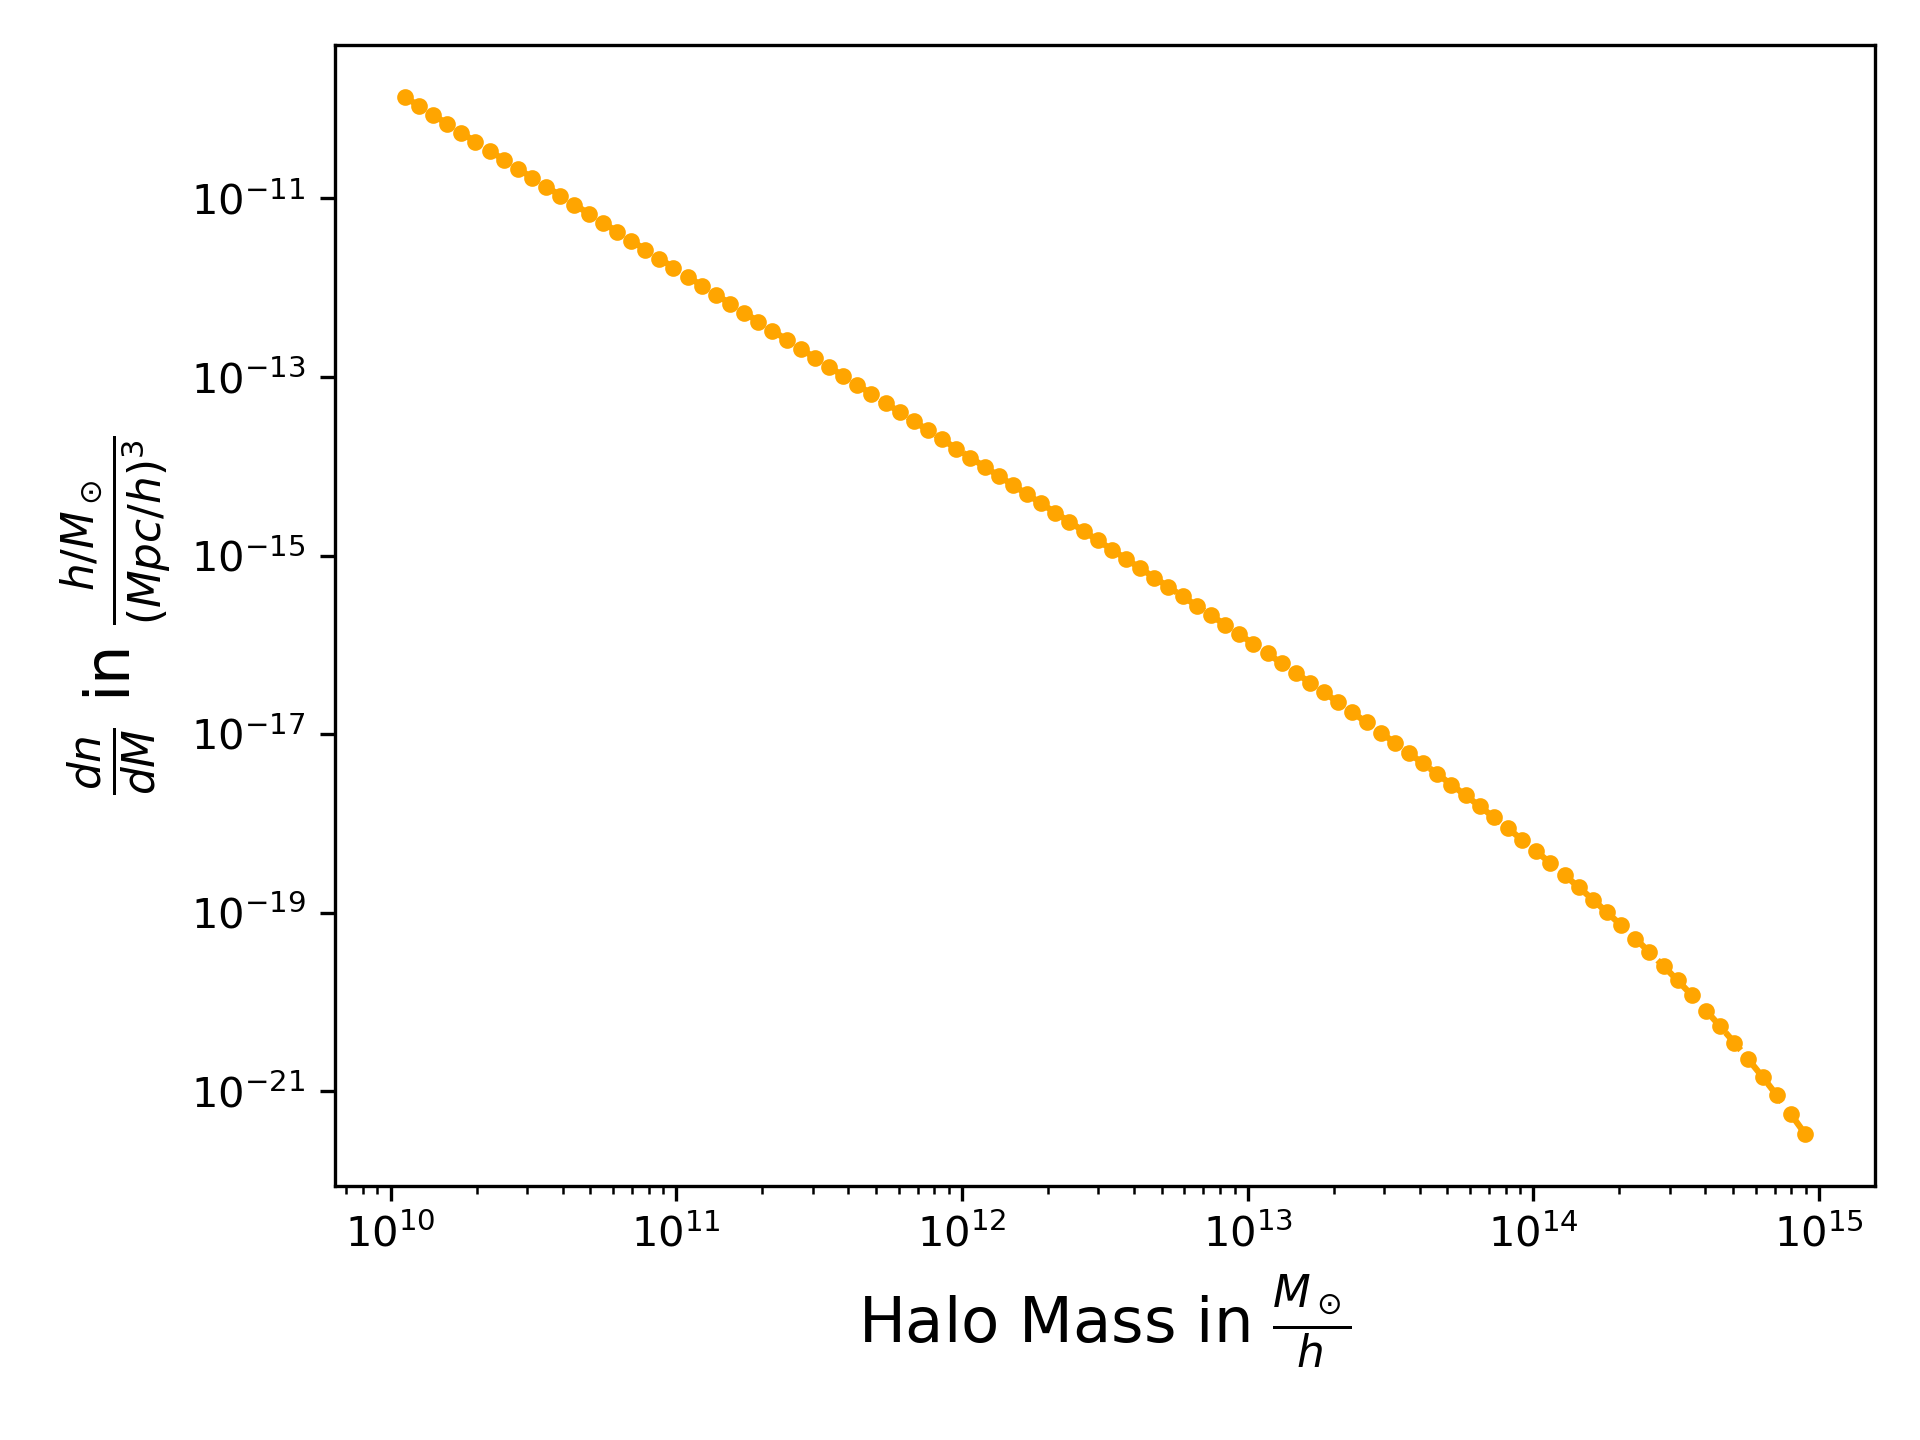
\includegraphics[width=7.5cm, clip]{Images/HMF.png}}
    \subfloat[{The dimensionless halo mass function }
        \label{HMF_dimless_plot}]{
        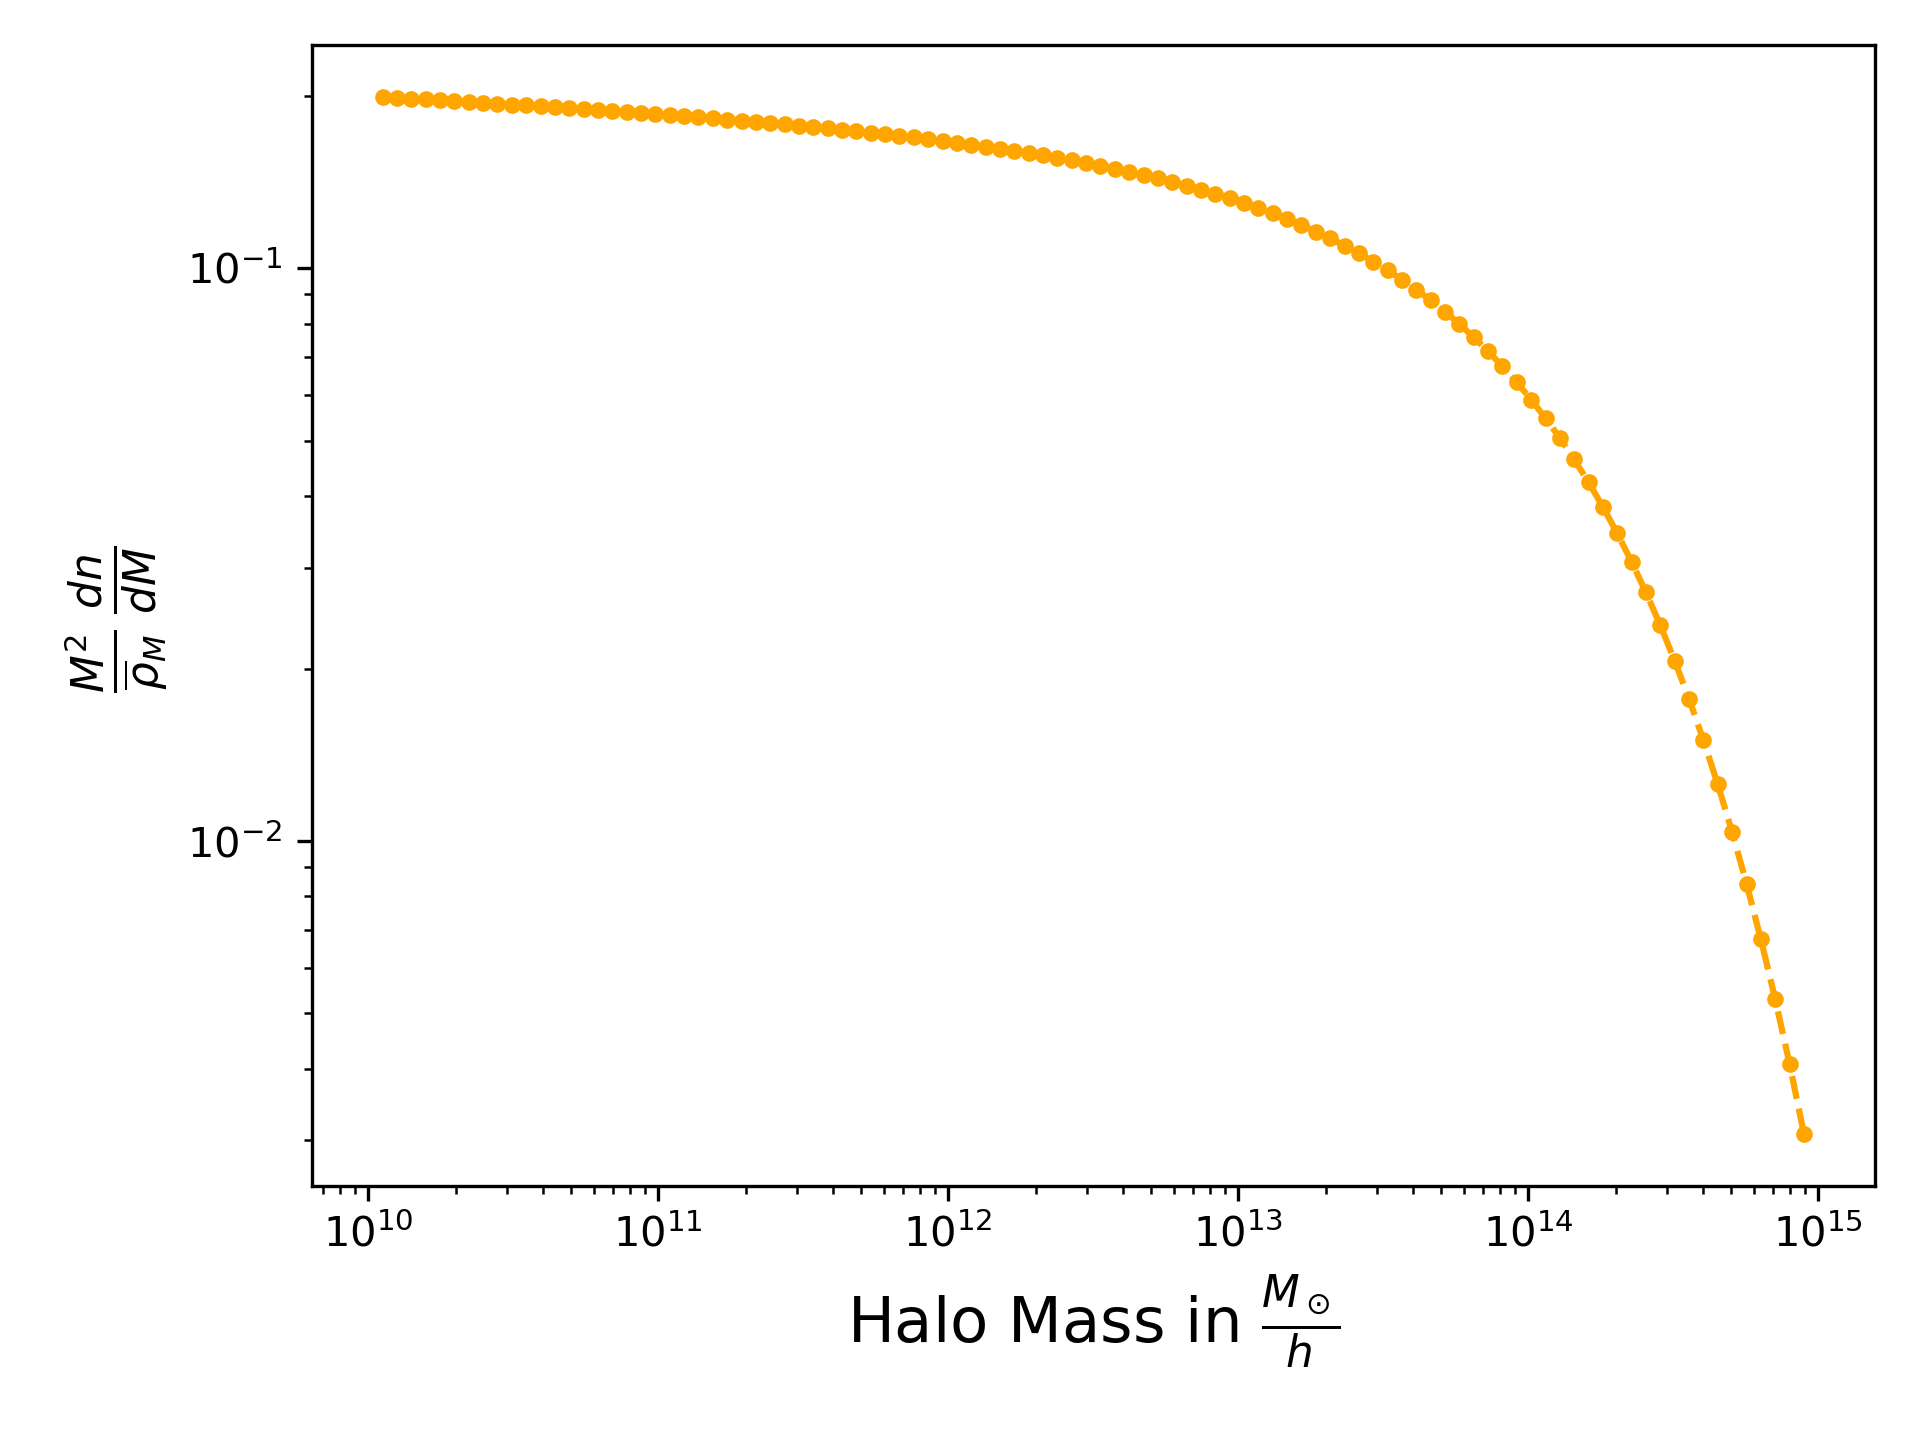
\includegraphics[width=7.5cm, clip]{Images/HMF_dimless.png}}
    \caption{Plots of the used HMFs.}
    \label{HMF_plots}
\end{figure} 


\section{Window Function}
\label{window_fct_section}

In Dall'Armi et al. \cite{dallarmi_dipole_2022} we see that the frequency dependence 
of the dipole comes from the evolution bias and the window function. The evolution 
bias accounts for the fact that more sources are created with time. The window 
function is used when we integrate the source functions over the redshift. 

\begin{equation}
\label{window_fct_int}
    \delta_{AGWB}(f_0, \hat{n})=\int dz \tilde{W}(f_0, z)\Delta_{AGWB}(f_0, \hat{n}, z)
\end{equation}


We can then Fourier and Legendre transform the GW density contrast:
\begin{equation}
    \delta_X(f_0, \vec{k}) = \int \frac{d^3\vec{x}}{(2\pi)^\frac{3}{2}} 
    \delta_X(f_0, \vec{x})
\end{equation}
\begin{equation}
    \Delta_l^X(k, f_0) = \int d\phi \int d\mu \mathcal{P}_l(\mu) 
    \delta^X(\vec{k}, f_0)
\end{equation}

From that, we can calculate the angular power spectrum using the primordial power 
spectrum:

\begin{equation}
    C_l^{XY} = 4\pi \int \frac{dk}{k} P(k) \Delta_l^X \Delta_l^{Y*}
\end{equation}

Here, X and Y can be the intrinsic, shot noise or kinematic (dipole) contribution.
Note, that this $\Delta$ is not the same as in equation \ref{window_fct_def}.

The window function depends upon others on the binary black hole merger rate.
\begin{equation}
\label{window}
    \tilde{W}(z, f_0)=\frac{f_0}{\rho_c c^2 \bar{\Omega}_{AGWB}(f_0)}
    \frac{R_{BBH}(z)}{(1+z)H(z)}\int d\vec{\theta}p(\vec{\theta})
    w(z, \vec{\theta}) \frac{dE_{GW}}{df_e d\Omega_e}(f_e, \vec{\theta})
\end{equation}

\begin{figure}[h]
    \centering
    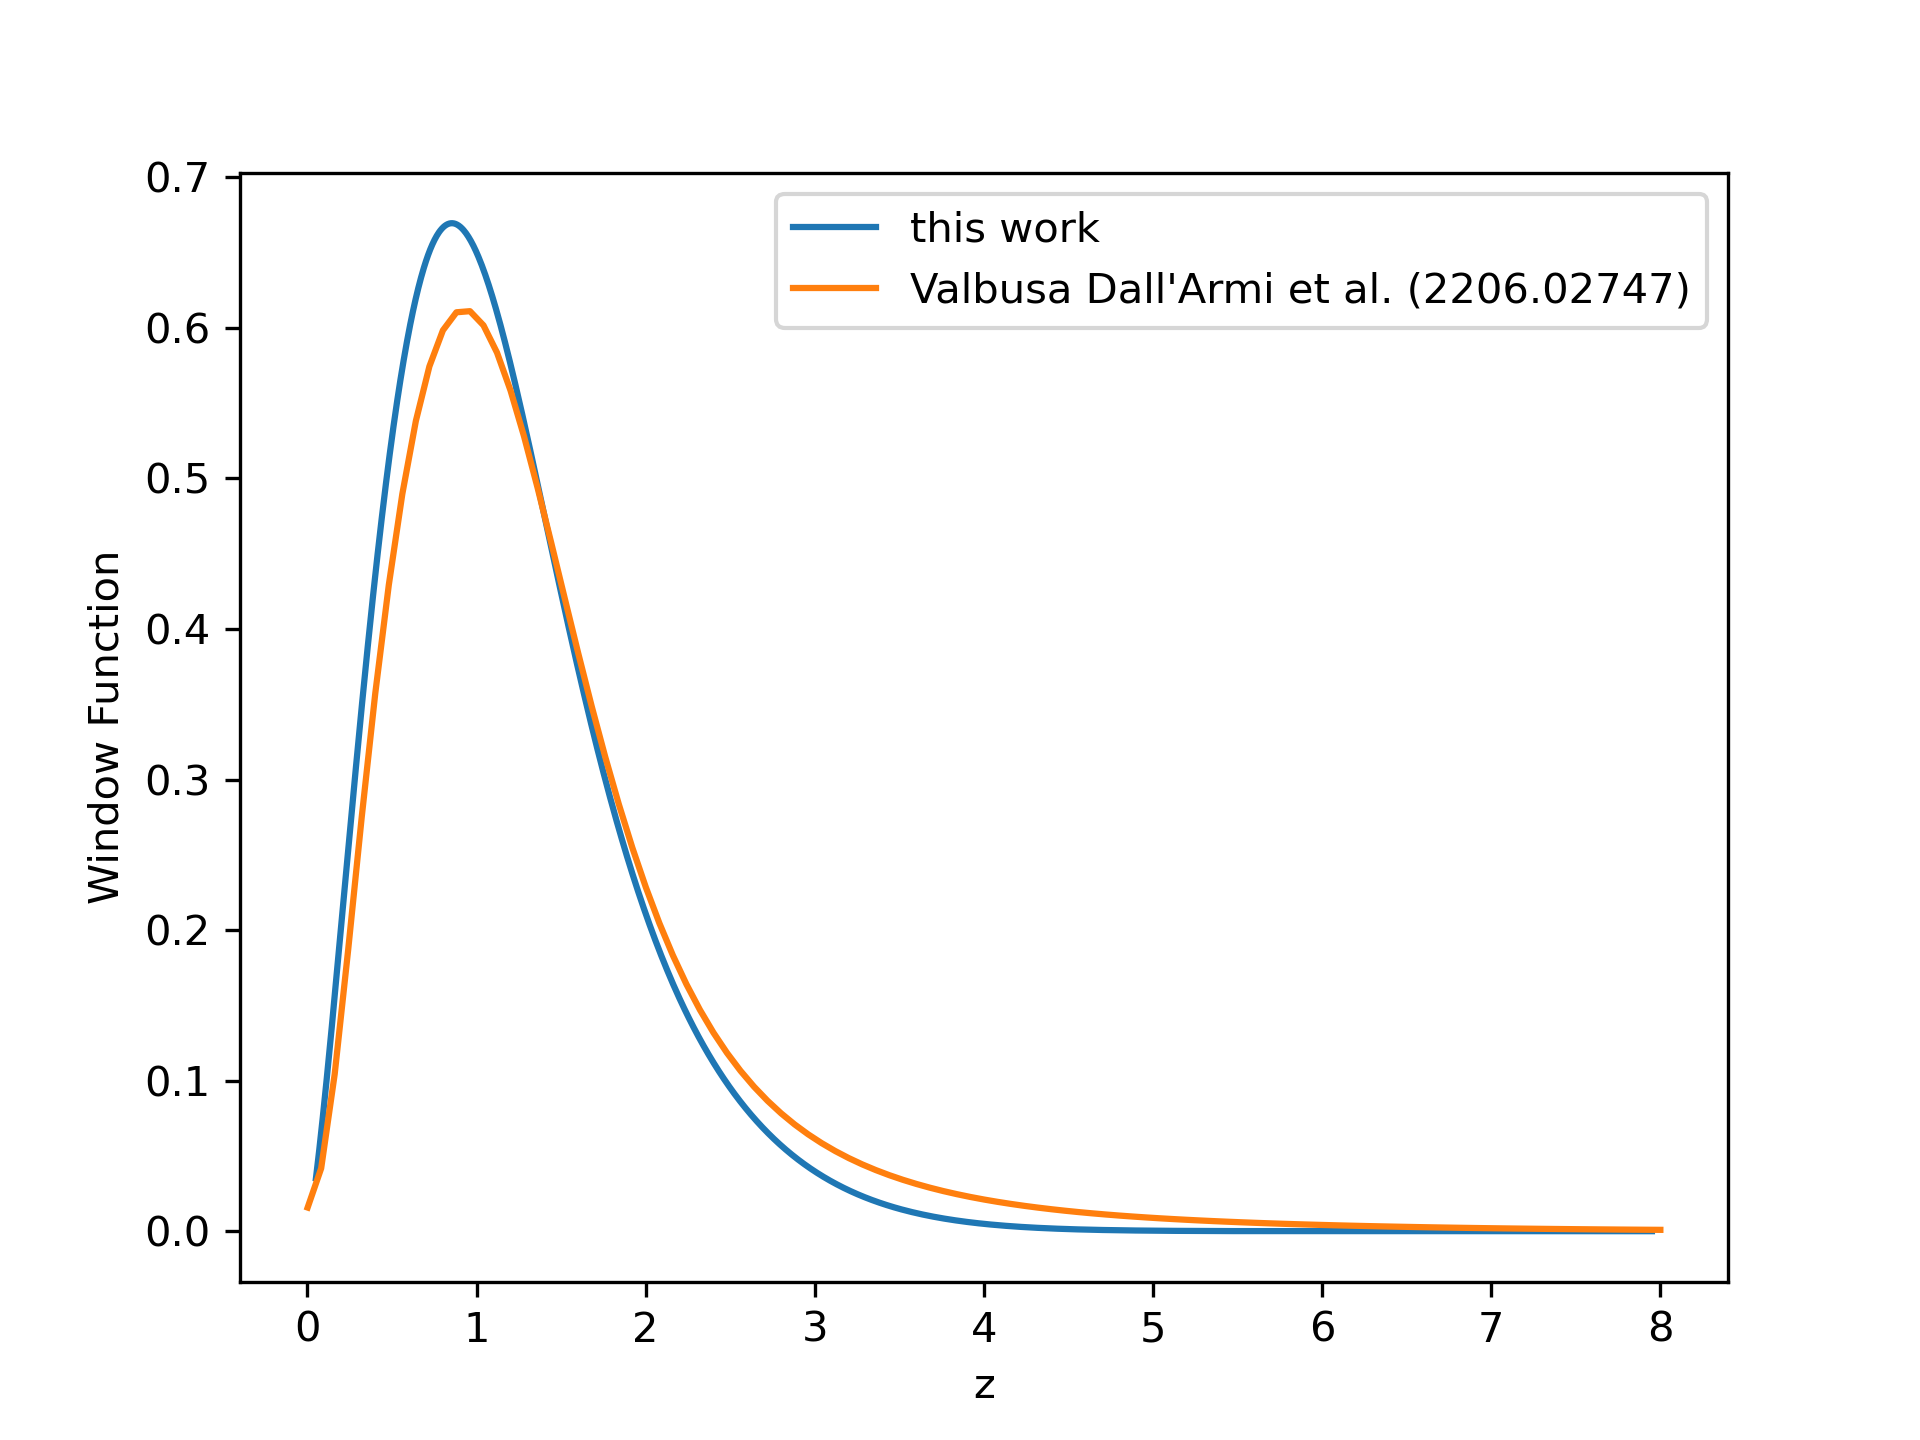
\includegraphics[width=0.8\linewidth]{Images/window_comparison.png}
    \caption{The final window function at 1 Hertz for this code in blue for comparison with \cite{dallarmi_dipole_2022} in orange.}
    \label{window_comparison}
\end{figure} 
%\vspace{-5cm}
\begin{figure}[h]
    \centering
    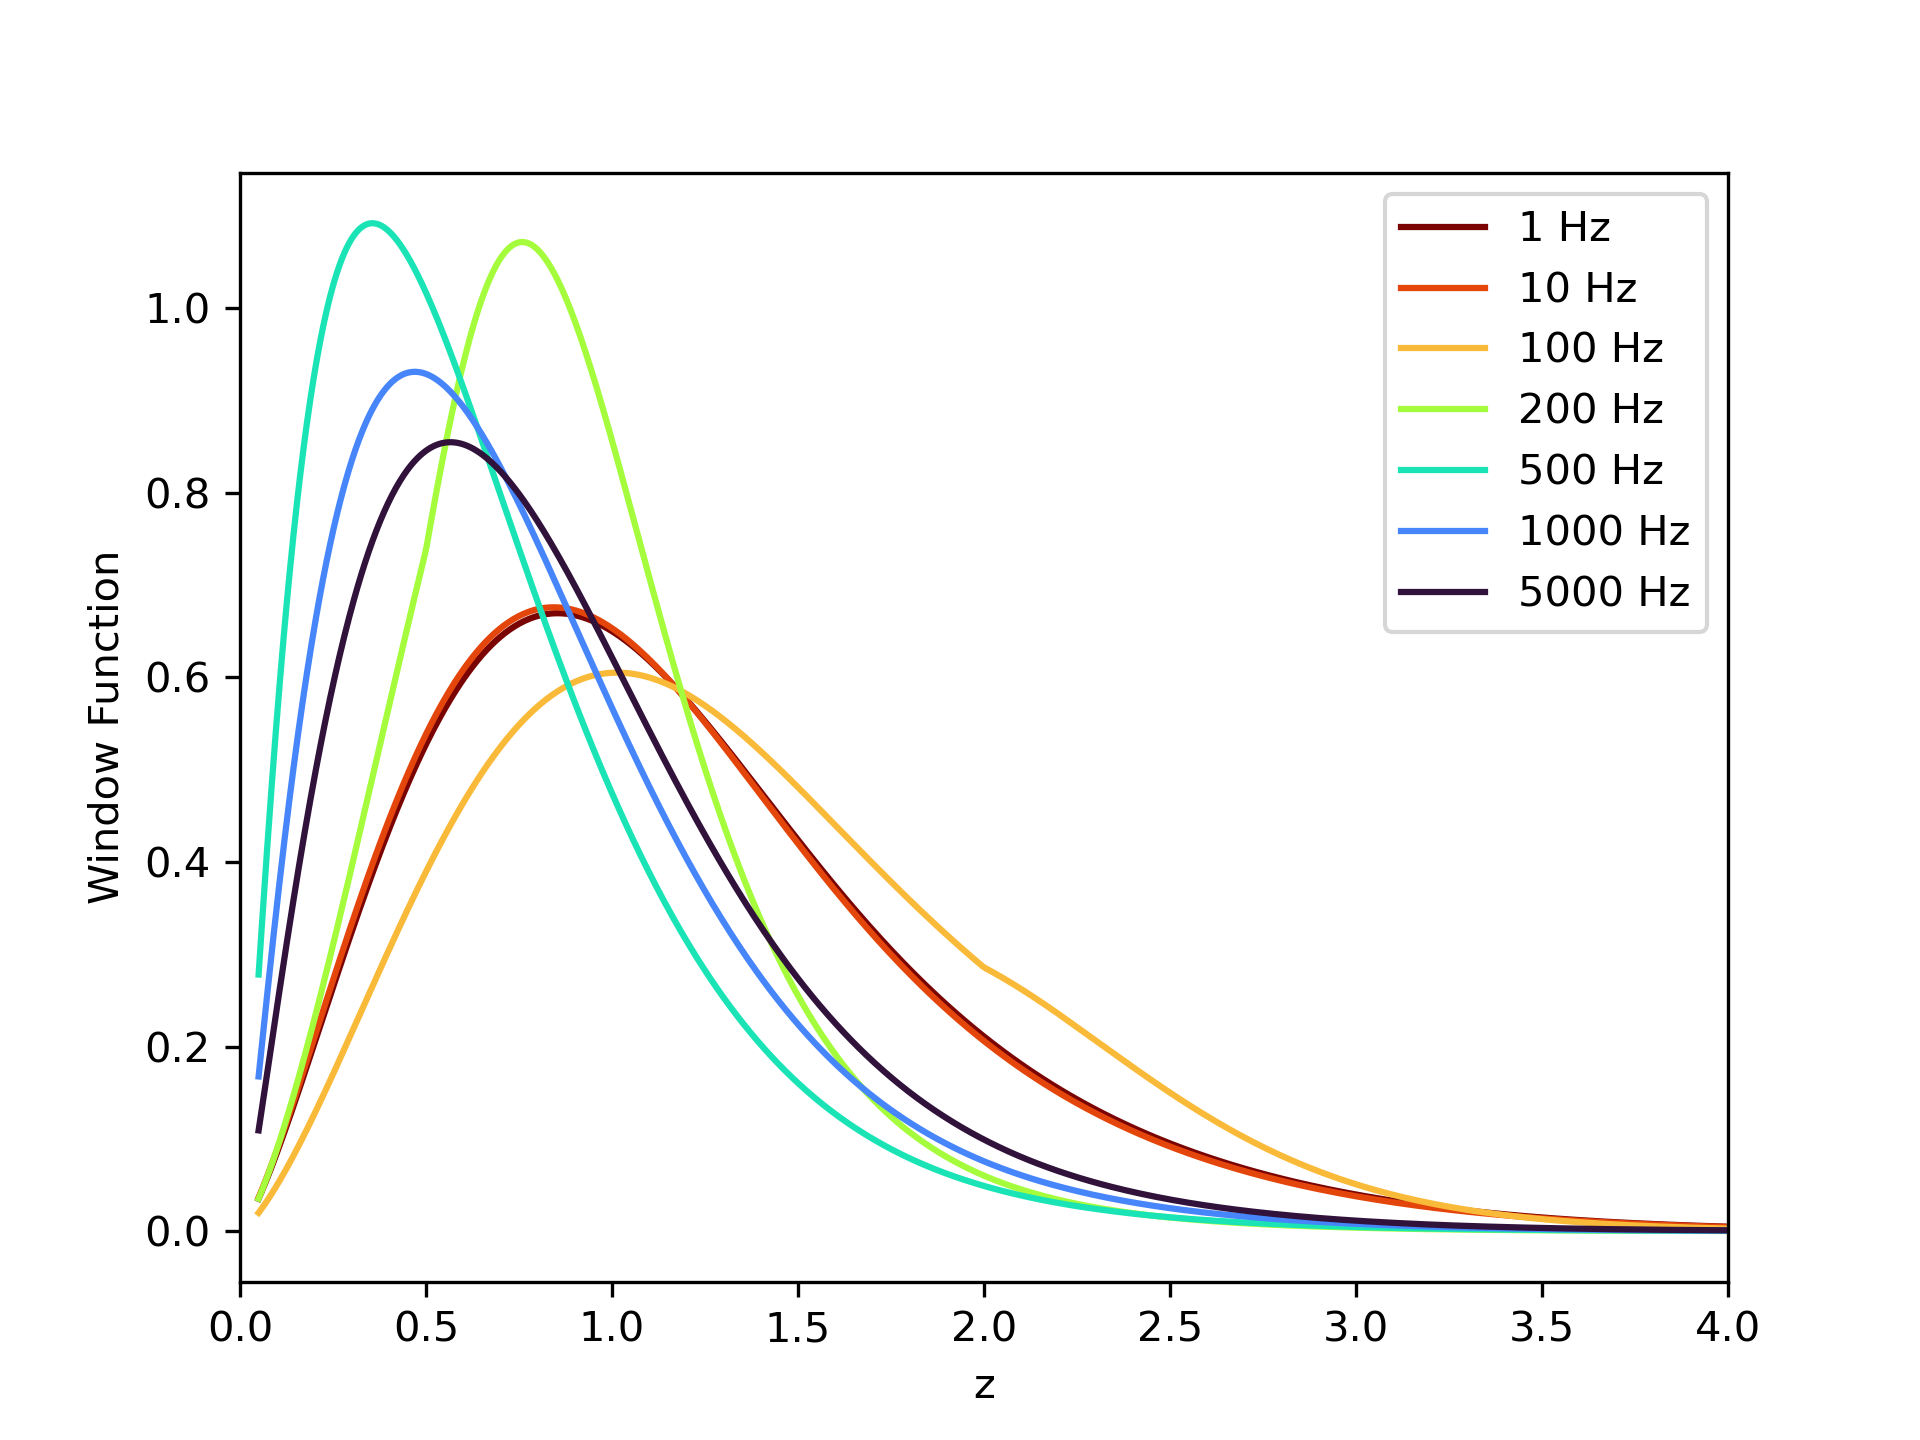
\includegraphics[width=1\linewidth]{Images/window_diff_frequencies.png}
    \caption{The window functions at different observed frequencies.}
    \label{window_frequencies}
\end{figure} 


\section{Evolution Bias}
\label{evo_bias_section}
The evolution bias accounts for the creation of new sources. This is why it depends on the redshift derivative of the merger rate and the energy spectrum of one merger. We can write this in terms of the derivative of the GW energy flux of the scale factor $a$.
\begin{equation}
    b_e(f_0, z) = \frac{d\ln(F)}{d\ln(a)}(f_0, z)
\end{equation}
\begin{equation}
    = -\frac{1+z}{F(f_0, z)}\frac{dF}{dz}(f_0, z)
\end{equation}
The energy flux of GW is a product of the energy spectrum of one binary, using the waveform by Ajith et al. \cite{ajith_inspiral-merger-ringdown_2011} and the merger rate of binary black holes as a function of redshift.
\begin{equation}
    F(f_0, z) = R_{BBH}(z) \frac{d E_{GW}}{df_e d\Omega_e}(f_0, z)
\end{equation}

It makes sense to use an Einstein-Boltzmann solver, like CLASS (cite), since the formalism of computing the angular power spectrum is similar to doing this for galaxy counts.

\section{Magnification Bias}
\textit{change style}


If one compares the contributions to $\Delta_l^{\rm{AGWB}}$ between {\tt CLASSgal} and the Dall'Armi paper \cite{dallarmi_dipole_2022}, the magnification bias has to be
 $s=\frac{2}{5}$ for the expressions to match. To find out why this is the case, 
 I tried some calculations with $\frac{dN}{dz}$, but could not match this value. 
 After reading the paper by Bertacca et al. \cite{bertacca_projection_2020} 
 (recommended by Lorenzo), one can see that they derive their expressions from 
 first principles without introducing the magnification bias separately. 